
\section{backup slides --- general}

\begin{frame}[fragile,label=arrayMissesOddEven1]{arrays and cache misses (1)}
\begin{lstlisting}
int array[1024]; // 4KB array
int even_sum = 0, odd_sum = 0;
for (int i = 0; i < 1024; i += 2) {
    even_sum += array[i + 0];
    odd_sum +=  array[i + 1];
}
\end{lstlisting}
    \begin{itemize}
        \item {\small
Assume everything but {\tt array} is kept in registers (and the compiler does not do
            anything funny).}
\item
How many \textit{data cache misses} on initially empty 2KB direct-mapped cache with 16B cache blocks?
    \end{itemize}
\end{frame}

\begin{frame}<1>[fragile,label=arrayMissesOddEven2]{arrays and cache misses (2)}
\begin{lstlisting}
int array[1024]; // 4KB array
int even_sum = 0, odd_sum = 0;
for (int i = 0; i < 1024; i += 2)
    even_sum += array[i + 0];
for (int i = 0; i < 1024; i += 2)
    odd_sum +=  array[i + 1];
\end{lstlisting}
    \begin{itemize}
        \item {\small
    Assume everything but {\tt array} is kept in registers (and the compiler does not do
    anything funny).
        }
    \item
How many \textit{data cache misses} on initially empty 2KB direct-mapped cache with 16B cache blocks?
            \only<2->{Would a set-associtiave cache be better?}
    \end{itemize}
\end{frame}

\begin{frame}[fragile,label=arrayMissesOddEven3]{arrays and cache misses (2b)}
\begin{lstlisting}
int array[1024]; // 4KB array
int even_sum = 0, odd_sum = 0;
for (int i = 0; i < 1024; i += 2)
    even_sum += array[i + 0];
for (int i = 0; i < 1024; i += 2)
    odd_sum +=  array[i + 1];
\end{lstlisting}
    \begin{itemize}
        \item {\small
    Assume everything but {\tt array} is kept in registers (and the compiler does not do
    anything funny).
        }
    \item
        How many \textit{data cache misses} on initially empty \myemph{4KB} direct-mapped cache with 16B cache blocks?
    \end{itemize}
\end{frame}

\begin{frame}[fragile,label=arrayMisses4]{arrays and cache misses (3)}
\begin{lstlisting}
int array[1024]; // 4KB array
int sum;
for (int i = 8; i < 1016; i += 1) {
    int local_sum = 0;
    for (int j = i - 8; j < i + 8; j += 1) {
        local_sum += array[i] * (j - i);
    }
    sum += (local_sum - array[i]);
}
\end{lstlisting}
    \begin{itemize}
        \item {\small
    Assume everything but {\tt array} is kept in registers (and the compiler does not do
    anything funny).
        }
    \item
        How many \textit{data cache misses} on initially empty \myemph{4KB} direct-mapped cache with 16B cache blocks?
    \end{itemize}
\end{frame}



\subsection{inclusive v exclusive}
\usetikzlibrary{patterns}
\begin{frame}{inclusive versus exclusive}
\begin{tikzpicture}
\tikzset{
    >=Latex,
    connect/.style={<->,ultra thick},
    cache/.style={draw,very thick},
    fill 1/.style={pattern color=blue!50!black,pattern=crosshatch},
    fill 2/.style={pattern color=orange,pattern=dots},
}
\node (l2 incl label) at (2.5, 6.5) {L2 inclusive of L1};
\node[font=\small,anchor=north,align=center] at (l2 incl label.south) {
    everything in L1 cache duplicated in L2 \\
    adding to L1 also adds to L2
};
\node[anchor=south]  at (1, 2) {L1 cache};
\node[anchor=south]  at (4, 4) {L2 cache};
\draw[cache] (0, 0) rectangle ++(2, 2);
\path[fill 1] (0, 0) rectangle ++(2, 2);
\path[fill 2] (3, -1.5) rectangle ++(2,1);
\path[fill 1] (3, -0.5) rectangle ++(2, .5);
\path[fill 2] (3, 0) rectangle ++(2,.25);
\path[fill 1] (3, 0.25) rectangle ++(2, .3);
\path[fill 2] (3, 0.55) rectangle ++(2,.65);
\path[fill 1] (3, 1.2) rectangle ++(2, .6);
\path[fill 2] (3, 1.8) rectangle ++(2,.2);
\path[fill 1] (3, 2) rectangle ++(2, .6);
\path[fill 2] (3, 2.6) rectangle ++(2,1.4);
\draw[cache] (3, -1.5) rectangle ++(2, 5.5);

\begin{scope}[xshift=8cm]
\node (l2 excl label) at (2.5, 6.5) {L2 exclusive of L1};
\node[font=\small,anchor=north,align=center] at (l2 excl label.south) {
    L2 contains different data than L1 \\
    adding to L1 must remove from L2 \\
    probably evicting from L1 adds to L2
};
\node[anchor=south]  at (1, 2) {L1 cache};
\node[anchor=south]  at (4, 4) {L2 cache};
\path[fill 1] (0, 0) rectangle ++(2, 2);
\draw[cache] (0, 0) rectangle ++(2, 2);
\draw[cache,fill 2] (3, -1.5) rectangle ++(2, 5.5);
\end{scope}
\begin{visibleenv}<2>
    \draw[overlay,red,very thick] (-1,-1.75) rectangle (6.25, 7);
    \fill[fill opacity=0.95,fill=white] (6.75, -1.75) rectangle (14, 7)
        node[midway,align=left,font=\small] {
            inclusive policy: \\
            no extra work on eviction \\
            but duplicated data \\
            ~ \\
            easier to explain when \\
            L$k$ shared by multiple L$(k-1)$ caches?
        };
\end{visibleenv}
\begin{visibleenv}<3>
    \draw[overlay,red,very thick] (6.75, -1.75) rectangle (14, 7);
    \fill[fill opacity=0.95,fill=white](-1,-1.75) rectangle (6.25, 7)
        node[midway,align=left,font=\small] {
            exclusive policy: \\
            avoid duplicated data \\
            sometimes called \textit{victim cache} \\
            (contains cache eviction victims) \\
            ~ \\
            makes less sense with multicore
        };
\end{visibleenv}
\end{tikzpicture}
\end{frame}



\subsection{tag/index/offset formulas}
\begin{frame}{Tag-Index-Offset formulas (direct-mapped)}
\begin{itemize}
\item (formulas derivable from prior slides)
\end{itemize}
\def\arraystretch{1.5}
\begin{tabular}{ll}
$S=2^s$ & number of sets \\
$s$  & (set) index bits \\
$B=2^b$ & block size \\
$b$ & (block) offset bits \\
$m$ & memory addreses bits \\
$t = m - (s+b)$ & tag bits \\
$C = B \times S$ & \myemph<2>{cache size} (if direct-mapped) \\
\end{tabular}
\end{frame}


\subsection{cut example?}
\usetikzlibrary{matrix,shapes.callouts,positioning,calc}
\begin{frame}<0>[fragile,label=pattern1]{example access pattern (1)}
\begin{tikzpicture}
\tikzset{
    v/.style={visible on=<#1->,alt=<#1>{red}},
    h/.style={alt=<#1>{red}},
}
\tikzset{
    tagColor/.style={color=green!60!black},
    dataColor/.style={color=blue!60!black},
    offsetColor/.style={color=yellow!30!black},
}
\matrix[tight matrix,
        nodes={font=\small,minimum height=.5cm,text depth=.1ex},
        column 1/.append style={nodes={font=\small\tt,text width=3.3cm,align=left}},
        row 1/.append style={nodes={font=\small\bfseries}},
        column 2/.append style={nodes={text width=1.3cm}},
        ] (pattern) {
    address (hex)\& result \\
    00000000 (00) \& |[v=4]| miss \\
    00000001 (01) \& |[v=5,h=12]| hit \\
    01100011 (63) \& |[v=6]| miss \\
    01100001 (61) \& |[v=7,h=12]| miss \\
    01100010 (62) \& |[v=8]| hit \\
    00000000 (00) \& |[v=9,h=12]| miss \\
    01100100 (64) \& |[v=10]| miss \\
};
\begin{pgfonlayer}{fg}
    \begin{visibleenv}<12-13>
        \node[my callout2=pattern-7-2.east,anchor=west] at ([xshift=1cm]pattern-7-2.east) {
            miss caused by \myemph{conflict}
        };
    \end{visibleenv}
\end{pgfonlayer}
\matrix[tight matrix,anchor=north west,
        nodes={font=\small\tt,text depth=.1ex,text height=1ex,minimum height=1cm},
        row 1/.append style={nodes={font=\small\bfseries,minimum height=.5cm}},
        column 1/.append style={nodes={draw=none,text width=1.2cm}},
        column 2/.append style={nodes={align=center,text width=1cm}},
        column 3/.append style={nodes={align=center,tagColor,text width=1.5cm}},
        column 4/.append style={nodes={text width=2.5cm,align=center,dataColor,
            text depth=2.3ex}},
        row 1 column 4/.append style={nodes={text depth=.1ex}},
        label={[font=\small]$2$ byte blocks, $4$ sets}] (cache) at ([xshift=.5cm]pattern.north east) {
    index \& valid \& tag \& value \\
    00 \& \zzx{1}{3}{0}\z{4}{1} \& \zz{4,5}{6}{00000}\zz{7}{8}{01100}\z{9}{00000} \& 
        \zz{4,5}{6}{mem[0x00] mem[0x01]}%
        \zz{7}{8}{mem[0x60] mem[0x61]}%
        \z{9}{mem[0x00] mem[0x01]}%
        \\
    01 \& \zzx{1}{5}{0}\z{6}{1} \& \z{6}{01100} \& \z{6}{mem[0x62] mem[0x63]} \\
    10 \& \zzx{1}{9}{0}\z{10}{1} \& \z{10}{01100} \& \z{10}{mem[0x64] mem[0x65]} \\
    11 \& 0 \& ~ \& ~ \\
};
\begin{visibleenv}<2->
    \node[anchor=north west,font=\small,align=left] (explain1) at ([yshift=-.5cm]pattern.south west) {
        $m = 8$ bit addresses \\ 
        $S=4=2^s$ sets \\
        $s=\myemph<2>{2}$ (set) index bits \\
    };
    \node[anchor=north west,font=\small,align=left] (explain2) at ([xshift=.5cm]explain1.north east) {
        $B=2=2^b$ byte block size \\
        $b=\myemph<2>{1}$ (block) offset bits \\
        $t = m - (s+b) = \myemph<2>{5}$ tag bits\\
    };
\end{visibleenv}
\begin{visibleenv}<3->
    \coordinate (tagTopLeft) at ([xshift=.1ex]pattern-2-1.north west);
    \coordinate (tagBottomLeft) at ([xshift=.1ex]pattern-8-1.south west);
    \coordinate (indexTopLeft) at ([xshift=5\oneZero]tagTopLeft);
    \coordinate (offsetTopLeft) at ([xshift=2\oneZero]indexTopLeft);
    \coordinate (offsetTopRight) at ([xshift=1\oneZero]offsetTopLeft);
    \coordinate (tagBottomRight) at (tagBottomLeft -| indexTopLeft);
    \coordinate (indexBottomRight) at (tagBottomLeft -| offsetTopLeft);
    \coordinate (offsetBottomRight) at (tagBottomLeft -| offsetTopRight);
    \fill[tagColor,opacity=0.3] (tagTopLeft) rectangle (tagBottomRight);
    \fill[offsetColor,opacity=0.3] (offsetTopLeft) rectangle (offsetBottomRight);
    \begin{scope}[every node/.style={anchor=north,text depth=.2ex,text height=1ex}]
        \node[tagColor,xshift=-.5cm] at ($(tagBottomLeft)!.5!(tagBottomRight)$) {
            tag
        };
        \node[xshift=-.2cm] at ($(tagBottomRight)!.5!(indexBottomRight)$) {
            index
        };
        \node[offsetColor,xshift=.6cm] at ($(indexBottomRight)!.5!(offsetBottomRight)$) {
            offset
        };
    \end{scope}
\end{visibleenv}

\end{tikzpicture}
\end{frame}


\subsection{benchmarking and cache results}
\usetikzlibrary{calc}

\begin{frame}{cache organization and miss rate}
\begin{itemize}
\item \myemph{depends on program}; one example:
\item SPEC CPU2000 benchmarks, 64B block size, LRU replacement
\item data cache miss rates:
{\small
\begin{tabular}{lrrrr}
Cache size & direct-mapped & 2-way & 8-way & fully assoc. \\
1KB & 8.63\% & 6.97\% & 5.63\% & 5.34\% \\
2KB & 5.71\% & 4.23\% & 3.30\% & 3.05\% \\
4KB & 3.70\% & 2.60\% & {2.03\%} & {1.90\%} \\
16KB & 1.59\% & 0.86\% & 0.56\% & 0.50\% \\
64KB & 0.66\% & 0.37\% & 0.10\% & 0.001\% \\
128KB & 0.27\% & 0.001\% & 0.0006\% & 0.0006\% \\
\end{tabular}
}
\end{itemize}
\imagecredit{
    \begin{tabular}{l}
    Data: Cantin and Hill, ``Cache Performance for SPEC CPU2000 Benchmarks'' \\
    \url{http://research.cs.wisc.edu/multifacet/misc/spec2000cache-data/}
    \end{tabular}
}
\end{frame}




\section{varying parameters exercise}
    % FIXME: put back?
\begin{frame}{exercise (1)}
    \begin{itemize}
    \item initial cache: 64-byte blocks, 64 sets, 8 ways/set
    \vspace{.5cm}
\item If we leave the other parameters listed above unchanged, which will probably reduce
    the number of \myemph{capacity misses} in a typical program? 
    (Multiple may be correct.) \\
    \begin{tabular}{ll}
        A. & quadrupling  the block size {\small (256-byte blocks, 64 sets, 8 ways/set)}\\
        B. & quadrupling the number of sets \\
        C. & quadrupling the number of ways/set\\
    \end{tabular}
    \end{itemize}
\end{frame}

\begin{frame}{exercise (2)}
    \begin{itemize}
    \item initial cache: 64-byte blocks, 8 ways/set, 64KB cache
    \vspace{.5cm}
    \item If we leave the other parameters listed above unchanged, which will probably reduce
          the number of \myemph{capacity misses} in a typical program? (Multiple may be correct.) \\
    \begin{tabular}{ll}
        A. & quadrupling the block size {\small (256-byte block, 8 ways/set, 64KB cache)}\\
        B. & quadrupling the number of ways/set \\
        C. & quadrupling the cache size \\
    \end{tabular}
    \end{itemize}
\end{frame}

\begin{frame}{exercise (3)}
    \begin{itemize}
    \item initial cache: 64-byte blocks, 8 ways/set, 64KB cache
    \vspace{.5cm}
    \item If we leave the other parameters listed above unchanged, which will probably reduce
          the number of \myemph{conflict misses} in a typical program? (Multiple may be correct.) \\
    \begin{tabular}{ll}
        A. & quadrupling the block size {\small (256-byte block, 8 ways/set, 64KB cache)}\\
        B. & quadrupling the number of ways/set \\
        C. & quadrupling the cache size \\
    \end{tabular}
    \end{itemize}
\end{frame}


\subsection{misc cache optimizations: prefetching}
    % FIXME: put back? (named in tradeoffs table)
\begin{frame}{prefetching}
    \begin{itemize}
    \item seems like we can't really improve cold misses\ldots
    \item have to have a miss to bring value into the cache?
    \vspace{.5cm}
    \item<2-> solution: don't require miss: `prefetch' the value before it's accessed
    \item<2-> remaining problem: how do we know what to fetch?
    \end{itemize}
\end{frame}

\begin{frame}{common access patterns}
    \begin{itemize}
    \item suppose recently accessed 16B cache blocks are at:
        \begin{itemize}
        \item 0x48010, 0x48020, 0x48030, 0x48040
        \end{itemize}
    \item guess what's accessed next
    \vspace{.5cm}
    \item<2-> common pattern with \myemph{instruction fetches} and \myemph{array accesses}
    \end{itemize}
\end{frame}

\begin{frame}{prefetching idea}
\begin{itemize}
\item look for sequential accesses
\item bring in guess at next-to-be-accessed value
\item if right: no cache miss (even if never accessed before)
\item if wrong: possibly evicted something else --- could cause more misses
    \begin{itemize}
    \item fortunately, sequential access guesses almost always right
    \end{itemize}
\end{itemize}
\end{frame}


\subsection{an old quiz question}
\usetikzlibrary{
    arrows.meta,
    decorations.pathreplacing,
    matrix,
}

\begin{frame}<0>[fragile,label=quizAccessSoln1]{quiz exercise solution}
\newcommand{\mywidth}{0.39}
\begin{tikzpicture}
    \foreach \offset in {-2,-1,0,1,2,...,31,32,33} {
        \draw[black!25,thin] (\offset * \mywidth, 0) rectangle ++(\mywidth, -.7);
    }
    \node[font=\large,anchor=east] at (-2 * \mywidth, -.5) {\ldots};
    \node[font=\large,anchor=west] at (34 * \mywidth, -.5) {\ldots};
    \begin{scope}
    \clip (-2.1 * \mywidth, .2) rectangle (34.1 * \mywidth, -.7);
    \foreach \offset/\name in {0/0,4/1,8/2,12/3,16/4,20/5,24/6,28/7,32/8} {
        \draw[thin,fill=blue!10] (\offset * \mywidth, 0) rectangle ++(\mywidth * 4, -.7)
            node[fill=none,opacity=1.0,black,midway,font=\fontsize{9}{10}\tt\selectfont] {array[\name]};
    }
    \foreach \offset in {-8,0,8,16,24,32} {
        \draw[ultra thick,red!30!black] (\offset * \mywidth, 0)
            rectangle ++(\mywidth * 8, -.7);
    }
    \end{scope}
        \draw[very thick, decorate, decoration={brace}] (8 * \mywidth, 0.05) -- ++(8 * \mywidth, 0)
            node[above,midway,align=center,font=\small] {one cache block \\
                                (set index 0)};
        \draw[very thick, decorate, decoration={brace}] (16 * \mywidth, 0.05) -- ++(8 * \mywidth, 0)
            node[above,midway,align=center,font=\small] {one cache block \\
                                (set index 1)};
        \draw[very thick, decorate, decoration={brace}] (24 * \mywidth, 0.05) -- ++(8 * \mywidth, 0)
            node[above,midway,align=center,font=\small] {one cache block \\
                                (set index 0)};
        \draw[very thick, decorate, decoration={brace}] (0 * \mywidth, 0.05) -- ++(8 * \mywidth, 0)
            node[above,midway,align=center,font=\small] {one cache block \\
                                (set index 1)};
    \tikzset{
        set both/.style={alt=<2-3>{nodes={fill=red!10}}},
        set 0/.style={
            alt=<2>{nodes={fill=red!10}},
            alt=<3>{opacity=0.1},
        },
        set 1/.style={
            alt=<3>{nodes={fill=red!10}},
            alt=<2>{opacity=0.1},
        },
    }
    \matrix[tight matrix,
        nodes={minimum height=0.5cm,font=\fontsize{8}{9}\selectfont},
        column 1/.append style={nodes={text width=4cm}},
        column 2/.append style={nodes={text width=5cm,font=\fontsize{10}{11}\tt\selectfont,set 0}},
        column 3/.append style={nodes={text width=5cm,font=\fontsize{10}{11}\tt\selectfont,set 1}},
        row 1/.append style={nodes={font=\fontsize{9}{10}\bfseries\selectfont}},
        row 2/.append style={set both},
        row 3/.append style={set 0},
        row 4/.append style={set 1},
        row 5/.append style={set 1},
        row 6/.append style={set 0},
        row 7/.append style={set 0},
        row 8/.append style={set 1},
        row 9/.append style={set 1},
        row 10/.append style={set 0},
        row 11/.append style={set 0},
        anchor=north west] at (-1, -1.7) {
        memory access \& set 0 afterwards \& set 1 afterwards \\ 
        --- \& (empty) \& (empty) \\
        read \lstinline|array[0]| (miss) \& \{array[0], array[1]\} \& (empty) \\
        read \lstinline|array[3]| (miss) \& \{array[0], array[1]\} \& \{array[2], array[3]\} \\
        read \lstinline|array[6]| (miss) \& \{array[0], array[1]\} \& \{array[6], array[7]\} \\
        read \lstinline|array[1]| (hit) \& \{array[0], array[1]\} \& \{array[6], array[7]\} \\
        read \lstinline|array[4]| (miss) \& \{array[4], array[5]\} \& \{array[6], array[7]\} \\
        read \lstinline|array[7]| (hit) \& \{array[4], array[5]\} \& \{array[6], array[7]\} \\
        read \lstinline|array[2]| (miss) \& \{array[4], array[5]\} \& \{array[2], array[3]\} \\
        read \lstinline|array[5]| (hit) \& \{array[4], array[5]\} \& \{array[6], array[7]\} \\
        read \lstinline|array[8]| (miss) \& \{array[8], array[9]\} \& \{array[6], array[7]\} \\
    };
\end{tikzpicture}
\end{frame}

\iftoggle{heldback}{}{
\againframe<1-3>{quizAccessSoln1}
}

\begin{frame}<0>[fragile,label=quizNotSoln]{not the quiz problem}
\newcommand{\mywidth}{0.39}
\begin{tikzpicture}
    \foreach \offset in {-2,-1,0,1,2,...,31,32,33} {
        \draw[black!25,thin] (\offset * \mywidth, 0) rectangle ++(\mywidth, -.7);
    }
    \node[font=\large,anchor=east] at (-2 * \mywidth, -.5) {\ldots};
    \node[font=\large,anchor=west] at (34 * \mywidth, -.5) {\ldots};
    \begin{scope}
    \clip (-2.1 * \mywidth, .2) rectangle (34.1 * \mywidth, -.7);
    \foreach \offset/\name in {0/0,4/1,8/2,12/3,16/4,20/5,24/6,28/7,32/8} {
        \draw[thin,fill=blue!10] (\offset * \mywidth, 0) rectangle ++(\mywidth * 4, -.7)
            node[fill=none,opacity=1.0,black,midway,font=\fontsize{9}{10}\tt\selectfont] {array[\name]};
    }
    \foreach \offset in {-8,0,8,16,24,32} {
        \draw[ultra thick,red!30!black] (\offset * \mywidth, 0)
            rectangle ++(\mywidth * 8, -.7);
    }
    \end{scope}
        \draw[very thick, decorate, decoration={brace}] (8 * \mywidth, 0.05) -- ++(8 * \mywidth, 0)
            node[above,midway,align=center,font=\small] {one cache block};
        \draw[very thick, decorate, decoration={brace}] (16 * \mywidth, 0.05) -- ++(8 * \mywidth, 0)
            node[above,midway,align=center,font=\small] {one cache bloc};
        \draw[very thick, decorate, decoration={brace}] (24 * \mywidth, 0.05) -- ++(8 * \mywidth, 0)
            node[above,midway,align=center,font=\small] {one cache block};
        \draw[very thick, decorate, decoration={brace}] (0 * \mywidth, 0.05) -- ++(8 * \mywidth, 0)
            node[above,midway,align=center,font=\small] {one cache block };
    \tikzset{
        set both/.style={alt=<2-3>{nodes={fill=red!10}}},
        set 0/.style={
            alt=<2>{nodes={fill=red!10}},
            alt=<3>{opacity=0.1},
        },
        set 1/.style={
            alt=<3>{nodes={fill=red!10}},
            alt=<2>{opacity=0.1},
        },
    }
    \matrix[tight matrix,
        nodes={minimum height=0.5cm,font=\fontsize{8}{9}\selectfont},
        column 1/.append style={nodes={text width=4cm}},
        column 2/.append style={nodes={text width=10cm,font=\fontsize{10}{11}\tt\selectfont}},
        row 1/.append style={nodes={font=\fontsize{9}{10}\bfseries\selectfont}},
        anchor=north west] (access matrix) at (-1, -1.7) {
        memory access \& single set with 2-ways, LRU first \\ 
        --- \& ---, --- \\
        read \lstinline|array[0]| (miss) \& ---, \{array[0], array[1]\} \\
        read \lstinline|array[3]| (miss) \& \{array[0], array[1]\}, \{array[2], array[3]\} \\
        read \lstinline|array[6]| (miss) \& \{array[2], array[3]\}, \{array[6], array[7]\} \\
        read \lstinline|array[1]| (miss) \& \{array[6], array[7]\}, \{array[0], array[1]\} \\
        read \lstinline|array[4]| (miss) \& \{array[0], array[1]\}, \{array[3], array[4]\} \\
        read \lstinline|array[7]| (miss) \& \{array[3], array[4]\}, \{array[6], array[7]\} \\
        read \lstinline|array[2]| (miss) \& \{array[6], array[7]\}, \{array[2], array[3]\} \\
        read \lstinline|array[5]| (miss) \& \{array[2], array[3]\}, \{array[5], array[6]\} \\
        read \lstinline|array[8]| (miss) \& \{array[5], array[6]\}, \{array[8], array[9]\} \\
    };
    \node[draw=red,very thick,anchor=south] at ([yshift=1mm]access matrix.north) {
        if 1-set 2-way cache instead of 2-set 1-way cache:
    };
\end{tikzpicture}
\end{frame}

\iftoggle{heldback}{}{
\againframe<1>{quizNotSoln}
}





\subsection{array misses exercises}

\subsection{sparse array miss exericse}
\begin{frame}[fragile,label=arrayMissesSparse2Alt]{C and cache misses (4)}
\begin{lstlisting}[language=C,style=small]
typedef struct {
    int a_value, b_value;
    int other_values[6];
} item;
item items[5];
int a_sum = 0, b_sum = 0;
for (int i = 0; i < 5; ++i)
    a_sum += items[i].a_value;
for (int i = 0; i < 5; ++i)
    b_sum += items[i].b_value;
\end{lstlisting}
    \begin{itemize}
        \item {\small
    Assume everything but {\tt items} is kept in registers (and the compiler does not do
    anything funny).
        }

    \end{itemize}
\end{frame}

\begin{frame}[fragile,label=arrayMissesSparse2bAlt]{C and cache misses (4, rewrite)}
\begin{lstlisting}[language=C,style=small]
int array[40]
int a_sum = 0, b_sum = 0;
for (int i = 0; i < 40; i += 8)
    a_sum += array[i];
for (int i = 1; i < 40; i += 8)
    b_sum += array[i];
\end{lstlisting}
    \begin{itemize}
        \item {\small
    Assume everything but {\tt array} is kept in registers (and the compiler does not do
    anything funny) and array starts at beginning of cache block.
        }
    \item
How many \textit{data cache misses} on a \myemph{2-way} set associative 128B cache with 16B cache blocks and
LRU replacement?
    \end{itemize}
\end{frame}


\begin{frame}[fragile,label=arrayMissesSparse2AltSoln1]{C and cache misses (4, solution pt 1)}
    \begin{itemize}
    \item ints 4 byte $\rightarrow$ array[0 to 3] and array[16 to 19] in same cache set
        \begin{itemize}
        \item 64B = 16 ints stored per way
        \item 4 sets total
        \end{itemize}
    \item accessing 0, 8, 16, 24, 32, 1, 9, 17, 25, 33
    \item<2-> 0 (set 0), 8 (set 2), 16 (set 0), 24 (set 2), 32 (set 0)
    \item<2-> 1 (set 0), 9 (set 2), 17 (set 0), 25 (set 2), 33 (set 0)
    \end{itemize}
\end{frame}

\begin{frame}[fragile,label=arrayMissesSparse2AltSoln2]{C and cache misses (4, solution pt 2)}
\begin{tabular}{lll}
access & set 0 after (LRU first) & result \\
--- & ---, --- \\
array[0] & ---, array[0 to 3] & miss \\
array[16] & array[0 to 3], array[16 to 19] & miss \\
array[32] & array[16 to 19], array[32 to 35] & miss \\
array[1] & array[32 to 35], array[0 to 3] & miss \\
array[17] & array[0 to 3], array[16 to 19] & miss \\
array[32] & array[16 to 19], array[32 to 35] & miss \\
\end{tabular}
6 misses for set 0
\end{frame}
\begin{frame}[fragile,label=arrayMissesSparse2AltSoln3]{C and cache misses (4, solution pt 3)}
\begin{tabular}{lll}
access & set 2 after (LRU first) & result \\
--- & ---, --- \\
array[8] & ---, array[8 to 11] & miss \\
array[24] & array[8 to 11], array[24 to 27] & miss \\
array[9] & array[8 to 11], array[24 to 27] & hit \\
array[25] & array[16 to 19], array[32 to 35] & hit \\
\end{tabular}
2 misses for set 1
\end{frame}


\section{alternate cache miss exericse}
\begin{frame}[fragile,label=arrayMissesSparse1Alt]{C and cache misses (3)}
\begin{lstlisting}[language=C,style=small]
typedef struct {
    int a_value, b_value;
    int other_values[10];
} item;
item items[5];
int a_sum = 0, b_sum = 0;
for (int i = 0; i < 5; ++i)
    a_sum += items[i].a_value;
for (int i = 0; i < 5; ++i)
    b_sum += items[i].b_value;
\end{lstlisting}
\begin{itemize}
    \item observation: 12 ints in struct: only first two used
    \item equivalent to accessing array[0], array[12], array[24], etc.
    \item \ldots then accessing array[1], array[13], array[25], etc.
\end{itemize}
\end{frame}


\begin{frame}[fragile,label=arrayMissesSparse1bAlt]{C and cache misses (3, rewritten?)}
\begin{lstlisting}[language=C,style=small]
int array[60];
int a_sum = 0, b_sum = 0;
for (int i = 0; i < 60; i += 12)
    a_sum += array[i];
for (int i = 1; i < 60; i += 12)
    b_sum += array[i];
\end{lstlisting}
    \begin{itemize}
        \item {\small
    Assume everything but {\tt array} is kept in registers (and the compiler does not do
    anything funny) and array at beginning of cache block.
        }
    \item
How many \textit{data cache misses} on a 128B two-way set associative cache with 16B cache blocks
and LRU replacement?
\item observation 1: first loop has 5 misses --- first accesses to blocks
\item observation 2: array[0] and array[1], array[12] and array[13], etc. in same cache block
    \end{itemize}
\end{frame}

\begin{frame}[fragile,label=arrayMissesSparse1bAltSoln]{C and cache misses (3, solution)}
    \begin{itemize}
    \item ints 4 byte $\rightarrow$ array[0 to 3] and array[16 to 19] in same cache set
        \begin{itemize}
        \item 64B = 16 ints stored per way
        \item 4 sets total
        \end{itemize}
    \item accessing array indices 0, 12, 24, 36, 48, 1, 13, 25, 37, 49
    \item<3-> 0 (set 0, array[0 to 3]), 12 (set 3), 24 (set 2), 36 (set 1), 48 (set 0)
        \begin{itemize}
        \item each set used at most twice
        \item no replacement needed
        \end{itemize}
    \item so access to 1, 21, 41, 61, 81 all hits:
        \begin{itemize}
        \item set 0 contains block with array[0 to 3]
        \item set 5 contains block with array[20 to 23]
        \item etc.
        \end{itemize}
    \end{itemize}
\end{frame}



\section{array misses and cache results (old sparse)}


\begin{frame}[fragile,label=arrayMissesSparse1]{C and cache misses (3)}
\begin{lstlisting}[language=C,style=small]
typedef struct {
    int a_value, b_value;
    int boring_values[126];
} item;
item items[8]; // 4 KB array
int a_sum = 0, b_sum = 0;
for (int i = 0; i < 8; ++i)
    a_sum += items[i].a_value;
for (int i = 0; i < 8; ++i)
    b_sum += items[i].b_value;
\end{lstlisting}
    \begin{itemize}
        \item {\small
    Assume everything but {\tt items} is kept in registers (and the compiler does not do
    anything funny).
        }
    \item
How many \textit{data cache misses} on a 2KB direct-mapped cache with 16B cache blocks?
    \end{itemize}
\end{frame}


\begin{frame}[fragile,label=arrayMissesSparse1b]{C and cache misses (3, rewritten?)}
\begin{lstlisting}[language=C,style=small]
item array[1024]; // 4 KB array
int a_sum = 0, b_sum = 0;
for (int i = 0; i < 1024; i += 128)
    a_sum += array[i];
for (int i = 1; i < 1024; i += 128)
    b_sum += array[i];
\end{lstlisting}
\end{frame}

\begin{frame}[fragile,label=arrayMissesSparse2]{C and cache misses (4)}
\begin{lstlisting}[language=C,style=small]
typedef struct {
    int a_value, b_value;
    int boring_values[126];
} item;
item items[8]; // 4 KB array
int a_sum = 0, b_sum = 0;
for (int i = 0; i < 8; ++i)
    a_sum += items[i].a_value;
for (int i = 0; i < 8; ++i)
    b_sum += items[i].b_value;
\end{lstlisting}
    \begin{itemize}
        \item {\small
    Assume everything but {\tt items} is kept in registers (and the compiler does not do
    anything funny).
        }
    \item
How many \textit{data cache misses} on a 4-way set associative 2KB direct-mapped cache with 16B cache blocks?
    \end{itemize}
\end{frame}


\subsection{set mapping (text)}
\begin{frame}[fragile,label=thinkStorage1]{thinking about cache storage (1)}
    \begin{itemize}
    \item 2KB direct-mapped cache with 16B blocks ---
    \item set 0: address 0 to 15\tikzmark{first}, (0 to 15) +\tikzmark{second} 2KB, (0 to 15) + 4KB, \ldots
        \begin{itemize}
        \item<3-> block at 0: \myemph<4>{array[0] through array[3]}
        \item<4-> block at 0+2KB: \myemph<4>{array[512] through array[515]}
        \end{itemize}
    \item set 1: address 16 to 31, (16 to 31) + 2KB, (16 to 31) + 4KB, \ldots \\
        \begin{itemize}
        \item<3-> block at 16: array[4] through array[7]
        \item<4-> block at 16+2KB: array[516] through array[519]
        \end{itemize}
    \item \ldots
    \item set 127: address 2032 to 2047, (2032 to 2047) + 2KB, \ldots
        \begin{itemize}
        \item<3-> block at 2032: array[508] through array[511]
        \item<4-> block at 2032+2KB: array[1020] through array[1023]
        \end{itemize}
    \end{itemize}
\end{frame}

\begin{frame}[fragile,label=thinkStorage2]{thinking about cache storage (2)}
    \begin{itemize}
    \item 2KB 2-way set associative cache with 16B blocks: block addresses --- 
    \item set 0: address 0\tikzmark{first}, 0 +\tikzmark{second} 2KB, 0 + 4KB, \ldots
        \begin{itemize}
        \item<2-> block at 0: \myemph<4>{array[0] through array[3]}
        \item<3-> block at 0+1KB: \myemph<4>{array[256] through array[259]}
        \item<3-> block at 0+2KB: \myemph<4>{array[512] through array[515]}
        \item<3-> \ldots
        \end{itemize}
    \item set 1: address 16, 16 + 2KB, 16 + 4KB, \ldots \\
        \begin{itemize}
        \item<2-> address 16: array[4] through array[7]
        \end{itemize}
    \item \ldots
    \item set 63: address 1008, 2032 + 2KB, 2032 + 4KB \ldots
        \begin{itemize}
        \item<2-> address 1008: array[252] through array[255]
        \end{itemize}
    \end{itemize}
\end{frame}


\subsection{array misses and skipping around}
\begin{frame}<1>[fragile,label=arrayMissesSkip]{misses with skipping}
\begin{lstlisting}
int array1[512]; int array2[512];
...
for (int i = 0; i < 512; i += 1)
    sum += array1[i] * array2[i];
}
\end{lstlisting}
    \begin{itemize}
        \item {\small
    Assume everything but {\tt array1}, {\tt array2} is kept in registers (and the compiler does not do
    anything funny).
        }
    \item
About how many \textit{data cache misses} on a 2KB direct-mapped cache with 16B cache blocks? \\
Hint: depends on relative placement of array1, array2
\end{itemize}
\end{frame}

\begin{frame}{best/worst case}
\begin{itemize}
\item \texttt{array1[i]} and \texttt{array2[i]} always different sets:
    \begin{itemize}
    \item 2 misses every 4 \texttt{i}
    \item = distance from array1 to array2 not multiple of \# sets $\times$ bytes/set
    \end{itemize}
\item \texttt{array1[i]} and \texttt{array2[i]} same sets:
    \begin{itemize}
    \item 2 misses every \texttt{i}
    \item = distance from array1 to array2 is multiple of \# sets $\times$ bytes/set
    \end{itemize}
\end{itemize}
\end{frame}

\begin{frame}{worst case in practice?}
    \begin{itemize}
    \item two rows of matrix?
    \item often sizeof(row) bytes apart
    \item if the row size is multiple of number of sets $\times$ bytes per block, oops!
    \end{itemize}
\end{frame}


\subsection{more complex array miss example}

\begin{frame}[fragile,label=arrayMisses4]{arrays and cache misses (3)}
\begin{lstlisting}
int sum; int array[1024]; // 4KB array
for (int i = 8; i < 1016; i += 1) {
    int local_sum = 0;
    for (int j = i - 8; j < i + 8; j += 1) {
        local_sum += array[i] * (j - i);
    }
    sum += (local_sum - array[i]);
}
\end{lstlisting}
    \begin{itemize}
        \item {\small
    Assume everything but {\tt array} is kept in registers (and the compiler does not do
    anything funny).
        }
    \item
        How many \textit{data cache misses} on initially empty \myemph{2KB} direct-mapped cache with 16B cache blocks?
    \end{itemize}
\end{frame}



\subsection{tag/index/offset exercise}
\subsubsection{setup}
\begin{frame}{Tag-Index-Offset exercise}

{\fontsize{12}{13}\selectfont
\begin{tabular}{ll}
$m$ & memory addreses bits (Y86-64: 64) \\
$E$ & number of blocks per set (``ways'') \\
$S=2^s$ & number of sets \\
$s$  & (set) index bits \\
$B=2^b$ & block size \\
$b$ & (block) offset bits \\
$t = m - (s+b)$ & tag bits \\
$C = B \times S \times E$ & cache size (excluding metadata) \\
\end{tabular}
}
    \begin{itemize}
        \item My desktop:
            \begin{itemize}
        \item L1 Data Cache: 32 KB, 8 blocks/set, 64 byte blocks
        \item L2 Cache: 256 KB, 4 blocks/set, 64 byte blocks
        \item L3 Cache: 8 MB, 16 blocks/set, 64 byte blocks
            \end{itemize}
        \begin{itemize}
            \item Divide the address {\tt 0x34567} into \myemph{tag}, \myemph{index}, \myemph{offset} for each cache.
        \end{itemize}
    \end{itemize} 
\end{frame}



\subsubsection{the exercise}
\providecommand{\KB}{\text{KB}}
\providecommand{\Byte}{\text{Byte}}

\begin{frame}{T-I-O exercise: L1}
\iftoggle{heldback}{}{
\def\arraystretch{1.1}
\begin{tabular}{llll}
quantity & value for L1\\\hline
block size (given) & $B=64\Byte$  \\ \hline
           & \multicolumn{3}{l}{$B=2^b$ ($b$: block offset bits)} \\ \pause
block offset bits & $b=\myemph{6}$ \\ \hline \pause
blocks/set (given) & $E=8$ \\ \hline
cache size (given) & $C = 32\KB = E \times B \times S$ \\ \hline \pause
           & \multicolumn{3}{l}{$S = \frac{C}{B\times E}$ ($S$: number of sets)} \\\pause
number of sets & $S = \frac{32\KB}{64\Byte\times 8} = \myemph{64}$ \\\hline \pause
               & \multicolumn{3}{l}{$S = 2^s$ ($s$: set index bits)} \\
set index bits & $s = \log_2(64) = \myemph{6}$ \\\hline
\end{tabular}
}
\end{frame}

\begin{frame}{T-I-O results}
\iftoggle{heldback}{}{
\begin{tabular}{llll}
~ & L1 & L2 & L3 \\ \hline
sets & 64 & 1024 & 8192 \\
block offset bits & 6 & 6 & 6 \\
set index bits & 6 & 10 & 13 \\
tag bits & \multicolumn{3}{c}{(the rest)} \\
\end{tabular}
}
\end{frame}

\begin{frame}{T-I-O: splitting}
\iftoggle{heldback}{}{
\begin{tabular}{llll}
~ & L1 & L2 & L3 \\ \hline
block offset bits & \myemph<1|handout:0>{6} & 6 & 6 \\
set index bits & 6 & 10 & 13 \\
tag bits & \multicolumn{3}{c}{(the rest)} \\
\end{tabular}
\begin{itemize}
\item {\tt 0x34567}:
\begin{tabular}{ccccc}
3 & 4 & 5 & 6 & 7 \\
\tt \myemph<4|handout:0>{0\myemph<7|handout:0>{011}} & \tt \myemph<4,5,7|handout:0>{0100} & 
\tt \myemph<3,5,7|handout:0>{0101} & 
\tt \myemph<3,5,7|handout:0>{01}\myemph<2|handout:0>{10} & 
\tt \myemph<2|handout:0>{0111} \\
\end{tabular}
\item bits 0-\myemph<1|handout:0>{5} (all offsets): {\tt \myemph<2>{100111}} = {\tt 0x27}
\only<3-4|handout:1>{
\item<3-> L1:
\begin{itemize}
    \item bits 6-11 (L1 set): {\tt \myemph<3>{01 0101}} = {\tt 0x15}
    \item bits 12- (L1 tag): \myemph<4>{\tt 0x34}
\end{itemize}
}
\only<5-6|handout:2>{
\item<5-> L2:
\begin{itemize}
    \item bits 6-15 (set for L2): {\tt \myemph<5>{01 0001 0101}} = {\tt 0x115}
    \item bits 16-: {\tt 0x3}
\end{itemize}
}
\only<7-|handout:3>{
\item<7-> L3:
\begin{itemize}
    \item bits 6-18 (set for L3): {\tt \myemph<7>{0 1101 0001 0101}} = {\tt 0xD15}
    \item bits 18-: {\tt 0x0} 
\end{itemize}
}
\end{itemize}
}
\end{frame}



\subsection{circuit diagram}
\usetikzlibrary{arrows.meta,circuits.logic.US,fit,matrix,positioning,shapes.callouts}

\begin{frame}{cache operation (associative)}
\begin{tikzpicture}[circuit logic US]
\tikzset{
    myline/.style={-latex,thick},
    myline thin/.style={-latex,thin},
    myline bus/.style={-latex,ultra thick},
    myline no arrow/.style={thick},
    offsetColor/.style={color=yellow!30!black},
    tagColor/.style={color=green!60!black},
    tagStoreFill/.style={fill=green!20},
    tagColorFill/.style={tagColor,fill=green!60!black},
    dataColor/.style={color=blue!60!black},
    dataColorFill/.style={tagColor,fill=blue!60!black},
    dataStoreFill/.style={fill=blue!20},
    triangle down/.style = {draw,regular polygon, regular polygon sides=3, shape border rotate=180},
}
\matrix[tight matrix,
        nodes={draw,
               font=\small\tt,
               text depth=0.2ex,
               text height=1.4ex,
        },
        row 1/.style={nodes={font=\small\bfseries}},
        column 1/.style={nodes={text width=1cm,align=center}},
        column 2/.style={nodes={text width=1cm,tagColor,tagStoreFill}},
        column 3/.style={nodes={text width=1.3cm,dataColor,dataStoreFill}},
        column 4/.style={nodes={text width=.1cm,draw=none}},
        column 5/.style={nodes={text width=1cm,align=center}},
        column 6/.style={nodes={text width=1cm,tagColor,tagStoreFill}},
        column 7/.style={nodes={text width=1.3cm,dataColor,dataStoreFill}},
        ] (cache) {
    valid \& tag \&  data \& ~ \& valid \& tag \& data\\
    1  \& 10 \& 00 11 \& ~ \& 1 \& 00 \& AA BB \\
    ~ \& ~ \& ~ \&   ~ \&  ~ \& ~ \& ~\\
    ~ \& ~ \& ~ \&   ~ \&  ~ \& ~ \& ~\\
    ~ \& ~ \& ~ \&   ~ \&  ~ \& ~ \& ~\\
    1 \&  11 \& B4 B5 \& ~ \& 1 \& 01 \& 33 44 \\
    ~ \& ~ \& ~ \&   ~ \&  ~ \& ~ \& ~\\
    ~ \& ~ \& ~ \&   ~ \&  ~ \& ~ \& ~\\
    ~ \& ~ \& ~ \&   ~ \&  ~ \& ~ \& ~\\
};
\begin{scope}[every node/.style={draw,rectangle,dashed,inner xsep=0pt,outer sep=0pt,font=\tt}]
\node (idx) at ([yshift=.5cm,xshift=-.3cm]cache.north west){100};
\node[left=0cm of idx,tagColor] (tag) {11};
\node[right=0cm of idx,offsetColor] (offset) {1};
\end{scope}
\draw[thick,dashed,-latex] (idx) |- (cache-6-1.west) node[near start,font=\small,fill=white,inner sep=2pt,xshift=-.3cm] {index};

%\begin{visibleenv}<2->
    \node[below=0.3cm of cache-9-2,draw,circle,inner sep=3pt] (comp1) {\small =};
    \node[below=1.4cm of cache-9-6,draw,circle,inner sep=3pt] (comp2) {\small =};
    %\coordinate(comp1Intersect) at ($(comp1) + (-.7cm,0.5cm)$);
    %\node[draw,circle,tagColorFill,inner sep=0pt,minimum width=1mm] at (comp1Intersect) {};
    \draw[tagColor,myline] (cache-9-2) -- (comp1);
    \draw[tagColor,myline] (cache-9-6) -- (comp2);

    %\draw[myline no arrow,tagColor] (tag) |- (comp1Intersect);
    %\draw[myline,tagColor] (comp1Intersect) |- (comp1);
    \draw[tagColor,myline] (tag) |- (comp2);
    \draw[tagColor,myline] (tag) |- (comp1) node[near start,font=\small,fill=white] {tag};
    %\draw[myline no arrow,tagColor] (comp1Intersect) |- (comp2Intersect);
    %\draw[myline,tagColor] (comp2Intersect) |- (comp2);

    \node[xshift=-.4cm,draw,below=1cm of cache-9-3,and gate,logic gate inputs=nn,label={[font=\scriptsize]center:AND}] (validCheck1) {};
    \node[xshift=-.4cm,draw,below=2.0cm of cache-9-7,and gate,logic gate inputs=nn,label={[font=\scriptsize]center:AND}] (validCheck2) {};
    \draw[myline] (comp1.south) |- (validCheck1.input 1);
    \draw[myline] (cache-9-1.south) |- (validCheck1.input 2);
    \draw[myline] (comp2.south) |- (validCheck2.input 1);
    \draw[myline] (cache-9-5.south) |- (validCheck2.input 2);
%\end{visibleenv}

\node[fit=(cache-6-1) (cache-6-7),inner sep=1pt,red,draw,line width=3pt] {};

%\node[draw,trapezium,inner xsep=0pt,outer sep=0pt,trapezium angle=75,below=.7cm of validCheck2,
%text width=5cm,shape border rotate=180,xshift=1.5cm] (mux) {};
%\draw[myline] (validCheck1.output) -| (buffer1.west);
%\draw[myline] (cache-9-3.south) -- (buffer1);
%\draw[myline] (buffer1.south) -- (bufEnd1);
\coordinate (outputData) at ([xshift=1.5cm,yshift=-.5cm]cache-9-7.south east);
\coordinate (beforeOutputData) at ([xshift=-.5cm]outputData);
\coordinate (outputHit1) at ([xshift=-1.5cm] beforeOutputData |- validCheck1.output);
\coordinate (outputHit2) at ([xshift=-1.5cm] beforeOutputData |- validCheck2.output);
%\begin{visibleenv}<2->
\node[or gate,logic gate inputs=nn,label={[font=\scriptsize]center:OR},anchor=output] (validCheckTotal)
    at ([xshift=1cm]$(outputHit1)!0.5!(outputHit2)$) {};
%\draw[myline] (validCheck1.output) -- (outputHit1) |- (validCheckTotal.input 1);
    \draw[myline no arrow] (validCheck1.output) -- ([xshift=-1pt]validCheck1.output -| cache-9-5.south);
    \draw[myline no arrow] ([xshift=1pt]validCheck1.output -| cache-9-5.south) -- 
                  ([xshift=-2pt]validCheck1.output -| cache-9-6.south);
    \draw[myline no arrow] ([xshift=2pt]validCheck1.output -| cache-9-6.south) -- (outputHit1);
    \draw[myline] (outputHit1) |- (validCheckTotal.input 1);
\draw[myline] (validCheck2.output) -- (outputHit2) |- (validCheckTotal.input 2);
\draw[myline] (validCheckTotal.output) -- ++(.5cm,0cm) node[right] {is hit? ({\tt 1})};
%\end{visibleenv}
%\begin{visibleenv}<3->
    \node[dataColor,draw,minimum width=.5cm,minimum height=1cm,mux,anchor=east,inputs=nn] (outputSelect) at ([xshift=-.2cm]beforeOutputData) {};
    \draw[myline] (outputHit1) -| (outputSelect.south);
    \fill[black] (outputHit1) circle (2pt);
    %\draw[myline,dataColor] (cache-9-3.south) |- (outputSelect.input 2);
        \draw[dataColor,myline no arrow] (cache-9-3.south) |- ([xshift=-1pt]cache-9-5.south |- outputSelect.input 2);
        \draw[dataColor,myline no arrow] ([xshift=1pt]cache-9-5.south |- outputSelect.input 2) --
                               ([xshift=-1pt]cache-9-6.south |- outputSelect.input 2);
        \draw[dataColor,myline] ([xshift=1pt]cache-9-6.south |- outputSelect.input 2) --
                               (outputSelect.input 2);
    \draw[myline,dataColor] (cache-9-7.south) |- (outputSelect.input 1);
    \draw[myline no arrow,dataColor] (outputSelect.output) -- (beforeOutputData);
    \node[draw,minimum width=.5cm,minimum height=1cm,mux,anchor=west,inputs=nn] (selectByte) at (outputData) {};
    \foreach \x in {1,2} {
        \draw[dataColor,myline thin] (beforeOutputData) |- (selectByte.input \x);
    };
    \draw[offsetColor,myline] (offset.east) -| (selectByte.north) node[very near start,fill=white,font=\small] {offset};
    \draw[dataColor,myline thin] (selectByte.output) -- ++(0.5cm,0cm) -- ++(0cm,0.5cm) node[above,align=center] {data\\({\tt B5})};
%\end{visibleenv}

\begin{visibleenv}<2-3>
\node[draw,red,thick,fit=(validCheck1)] {};
\node[draw,red,thick,fit=(comp1)] {};
\draw[red,thick,dashed,-Latex] (validCheck1.output) -| (outputSelect.south);
\end{visibleenv}
\begin{visibleenv}<3>
\draw[thick,red,-Latex] (outputSelect.input 2) -- (outputSelect.output);
\end{visibleenv}
\end{tikzpicture}
% FIXME: place diagram here
\end{frame}




\subsection{backup slides --- cache performance}
\begin{frame}{backup slides --- cache performance}
\end{frame}

\subsection{AMAT}
\begin{frame}{average memory access time}
    \begin{itemize}
    \item $\text{AMAT} = \text{hit time} + \text{miss penalty} \times \text{miss rate}$
        \begin{itemize}
        \item or $\text{AMAT} = \text{hit time} \times \text{hit rate} + \text{miss time} \times \text{miss rate}$
        \end{itemize}
    \item effective speed of memory
    \end{itemize}
\end{frame}


\subsubsection{exercise: AMAT (simple case)}
\begin{frame}{AMAT exercise (1)}
\begin{itemize}
\item 90\% cache hit rate
\item hit time is 2 cycles
\item 30 cycle miss penalty
\item what is the average memory access time?
\item<2-> \iftoggle{heldback}{}{5 cycles}
\vspace{.5cm}
\item suppose we could increase hit rate by increasing its size, but it would increase the hit time to 3 cycles
\item how much do we have to increase the hit rate for this to not increase AMAT?
\item<3-> \iftoggle{heldback}{}{to miss rate of 2/30 $\rightarrow$ to approx 93\% hit rate}
\end{itemize}
\end{frame}


\subsubsection{exercise: multi-level cache AMAT}
\begin{frame}{exercise: AMAT and multi-level caches}
\begin{itemize}
\item suppose we have L1 cache with
    \begin{itemize}
    \item 3 cycle hit time
    \item 90\% hit rate
    \end{itemize}
\item and an L2 cache with
    \begin{itemize}
    \item 10 cycle hit time
    \item 80\% hit rate (for accesses that make this far)
    \item (assume all accesses come via this L1)
    \end{itemize}
\item and main memory has a 100 cycle access time
\item assume when there's an cache miss, the next level access starts after the hit time
    \begin{itemize}
    \item e.g. an access that misses in L1 and hits in L2 will take 10+3 cycles
    \end{itemize}
\item what is the average memory access time for the L1 cache?
\begin{itemize}
\item<2-> \iftoggle{heldback}{~}{$3 + 0.1\cdot(\myemph<3>{10 + 0.2\cdot100}) = 6$ cycles}
\item<3-> \iftoggle{heldback}{~}{L1 miss penalty is $10 + 0.2\cdot100 = 30$ cycles}
\end{itemize}
\end{itemize}
\end{frame}


\subsection{less precise approxmation}
\begin{frame}{approximate miss analysis}
    \begin{itemize}
    \item very tedious to precisely count cache misses
        \begin{itemize}
        \item even more tedious when we take advanced cache optimizations into account
        \end{itemize}
    \vspace{.5cm}
    \item instead, approximations:
    \item \myemph<2>{good or bad temporal/spatial locality}
        \begin{itemize}
        \item good temporal locality: value stays in cache
        \item good spatial locality: use all parts of cache block
        \end{itemize}
    \item with nested loops: what does inner loop use?
        \begin{itemize}
        \item intuition: values used in inner loop loaded into cache once 
        \item (that is, once each time the inner loop is run)
        \item \ldots if they can all fit in the cache
        \end{itemize}
    \end{itemize}
\end{frame}


% FIXME: cache performance intro
\subsection{warmup: locality exercise}  % FIXME: move earlier?
\begin{frame}[fragile,label=localityExercise1]{locality exercise (1)}
\lstset{language=C,style=small}
\begin{lstlisting}
/* version 1 */
for (int i = 0; i < N; ++i)
    for (int j = 0; j < N; ++j)
        A[i] += B[j] * C[i * N + j]

/* version 2 */
for (int j = 0; j < N; ++j)
    for (int i = 0; i < N; ++i)
        A[i] += B[j] * C[i * N + j];
\end{lstlisting}
exercise: which has better temporal locality in A? in B? in C? \\
how about spatial locality?
\end{frame}



\subsection{warmup: miss counting}
\begin{frame}[fragile,label=missCountingEx]{exercise: miss estimating (1)}
\lstset{language=C,style=small}
\begin{lstlisting}
for (int i = 0; i < N; ++i)
    for (int j = 0; j < N; ++j)
        A[i] += B[j] * C[i * N + j]
\end{lstlisting}
\begin{itemize}
\item Assume: 4 array elements per block, N very large, nothing in cache at beginning.\\
\item Example: $N/4$ estimated misses for A accesses:
\begin{itemize}
\item A[i] should always be hit on all but first iteration of inner-most loop.
\item first iter: A[i] should be hit about 3/4s of the time (same block as A[i-1] that often)
\end{itemize}
\item Exericse: estimate \# of misses for B, C
\end{itemize}
\end{frame}



\subsection{2D arrays in C}
\begin{frame}[fragile,label=flatMatrix]{a note on matrix storage}
\begin{itemize}
\item $A$ --- $N\times N$ matrix
\item represent as \myemph{array}
\item makes dynamic sizes easier:
\end{itemize}
\lstset{style=small,language=C,escapechar=@}
\begin{lstlisting}
float A_2d_array[N][N];
float *A_flat = malloc(N * N);

A_flat[i * N + j] === A_2d_array[i][j]
\end{lstlisting}
\end{frame}

\begin{frame}{convertion re: rows/columns}
\begin{itemize}
\item going to call the first index rows
\item $A_{i,j}$ is A row i, column j
\item rows are stored together
\vspace{.5cm}
\item this is an arbitrary choice
\end{itemize}
\end{frame}

% FIXME: cache blocks and 2D array
\usetikzlibrary{fit,matrix}
\begin{frame}{5x5 array and 4-element cache blocks}
\begin{tikzpicture}
\tikzset{
    cb1/.style={
        alt={<2,5>{fill=red!15}},
    },
    cb2/.style={
        alt={<3,5>{fill=orange!20}},
    },
    cb3/.style={
        alt={<4,5>{fill=yellow!20}},
    },
    cb4/.style={
        alt=<5>{fill=green!15},
    },
    cb5/.style={
        alt=<5>{fill=blue!15},
    },
    cb6/.style={
        alt=<5>{fill=violet!15},
    },
    cb7/.style={
        alt=<5>{fill=magenta!20},
    },
}
\matrix[tight matrix,nodes={font=\fontsize{9}{10}\selectfont,text width=2.5cm}] (a) {
    |[cb1]| \tt array[0*5 + 0] \&
    |[cb1]| \tt array[0*5 + 1] \&
    |[cb1]| \tt array[0*5 + 2] \&
    |[cb1]| \tt array[0*5 + 3] \&
    |[cb2]| \tt array[0*5 + 4] \\
    |[cb2]| \tt array[1*5 + 0] \&
    |[cb2]| \tt array[1*5 + 1] \&
    |[cb2]| \tt array[1*5 + 2] \&
    |[cb3]| \tt array[1*5 + 3] \&
    |[cb3]| \tt array[1*5 + 4] \\
    |[cb3]| \tt array[2*5 + 0] \&
    |[cb3]| \tt array[2*5 + 1] \&
    |[cb4]| \tt array[2*5 + 2] \&
    |[cb4]| \tt array[2*5 + 3] \&
    |[cb4]| \tt array[2*5 + 4] \\
    |[cb4]| \tt array[3*5 + 0] \&
    |[cb5]| \tt array[3*5 + 1] \&
    |[cb5]| \tt array[3*5 + 2] \&
    |[cb5]| \tt array[3*5 + 3] \&
    |[cb5]| \tt array[3*5 + 4] \\
    |[cb6]| \tt array[4*5 + 0] \&
    |[cb6]| \tt array[4*5 + 1] \&
    |[cb6]| \tt array[4*5 + 2] \&
    |[cb6]| \tt array[4*5 + 3] \&
    |[cb7]| \tt array[4*5 + 4] \\
};
\begin{visibleenv}<2>
\node[align=left,anchor=north] at ([yshift=-1cm]a.south) {
    if array starts on cache block \\
    first cache block = first elements \\
    all together in one row!
};
\end{visibleenv}
\begin{visibleenv}<3>
\node[align=left,anchor=north] at ([yshift=-1cm]a.south) {
    second cache block: \\
    1 from row 0 \\
    3 from row 1 \\
};
\end{visibleenv}
\begin{visibleenv}<5>
\node[align=left,anchor=north] at ([yshift=-1cm]a.south) {
    generally: cache blocks contain data from 1 or 2 rows \\
    $\rightarrow$ better performance from reusing rows
};
\end{visibleenv}
\end{tikzpicture}
\end{frame}


\subsection{matrix multiply and loop orders}
\begin{frame}[fragile,label=matrixMult]{matrix multiply}
\[ C_{ij} = \sum_{k=1}^n A_{ik}\times B_{kj} \]
\lstset{language=C,style=small}
\begin{lstlisting}
/* version 1: inner loop is k, middle is j */
for (int i = 0; i < N; ++i)
  for (int j = 0; j < N; ++j)
    for (int k = 0; k < N; ++k)
      C[i * N + j] += A[i * N + k] * B[k * N + j];
\end{lstlisting}
\end{frame}

%\begin{frame}[fragile,label=matrixSquare]{matrix squaring}
\[ B_{ij} = \sum_{k=1}^n A_{ik}\times A_{kj} \]
\lstset{language=C,style=small}
\begin{lstlisting}
/* version 1: inner loop is k, middle is j */
for (int i = 0; i < N; ++i)
  for (int j = 0; j < N; ++j)
    for (int k = 0; k < N; ++k)
      B[i * N + j] += A[i * N + k] * A[k * N + j];
\end{lstlisting}
\end{frame}

\begin{frame}<1>[fragile,label=matrixMultTwoVersions]{matrix multiply}
\[ C_{ij} = \sum_{k=1}^n A_{ik}\times B_{kj} \]
\lstset{
    style=small,
    language=C,
    moredelim=**[is][\btHL<2>]{~2}{~},
    moredelim=**[is][\btHL<3>]{~3}{~},
    moredelim=**[is][\btHL<4>]{~4}{~},
}
\begin{lstlisting}
/* version 1: inner loop is k, middle is j*/
for (int i = 0; i < N; ++i)
  for (int j = 0; j < N; ++j)
    for (int k = 0; k < N; ++k)
      ~2C[i*N+j]~ += A[i * N + k] * B[k * N + j];

/* version 2: outer loop is k, middle is i */
for (int k = 0; k < N; ++k)
  for (int i = 0; i < N; ++i)
    for (int j = 0; j < N; ++j)
      C[i*N+j] += ~2A[i * N + k]~ * B[k * N + j];
\end{lstlisting}
\end{frame}


\begin{frame}{loop orders and locality}
\begin{itemize}
\item loop body: $C_{ij} += A_{ik}B_{kj}$
\item $ki\myemph<2>{j}$ order: $C_{i\myemph<2>{j}}$, $B_{k\myemph<2>{j}}$ have \myemph<1>{spatial locality}
\item $kij$ order: $A_{ik}$ has \myemph<1>{temporal locality}
\item \ldots{} better than \ldots{}
\item $ij\myemph<2>{k}$ order: $A_{i\myemph<2>{k}}$ has spatial locality
\item $ijk$ order: $C_{ij}$ has temporal locality
\end{itemize}
\end{frame}

\begin{frame}[fragile,label=matrixMultTwoVersionsHilite]{matrix multiply}
\[ C_{ij} = \sum_{k=1}^n A_{ik}\times B_{kj} \]
\lstset{
    style=small,
    language=C,
    moredelim=**[is][\btHL<2>]{~2}{~},
    moredelim=**[is][\btHL<3>]{~3}{~},
    moredelim=**[is][\btHL<4>]{~4}{~},
}
\begin{lstlisting}
/* version 1: inner loop is k, middle is j*/
for (int i = 0; i < N; ++i)
  for (int j = 0; j < N; ++j)
    for (int k = 0; k < N; ++k)
      ~3C[i*N+j]~ += A[i * N + ~2k~] * B[k * N + j];

/* version 2: outer loop is k, middle is i */
for (int k = 0; k < N; ++k)
  for (int i = 0; i < N; ++i)
    for (int j = 0; j < N; ++j)
      C[i*N+~2j~] += ~3A[i * N + k]~ * B[k * N + ~2j~];
\end{lstlisting}
\end{frame}

\subsubsection{exercise: which order?}
\begin{frame}<1>[fragile,label=matrixMultLocalityEx]{which is better?}
\[ C_{ij} = \sum_{k=1}^n A_{ik}\times B_{kj} \]
\lstset{
    style=smaller,
    language=C,
    moredelim=**[is][\btHL<2>]{~2}{~},
    moredelim=**[is][\btHL<3>]{~3}{~},
    moredelim=**[is][\btHL<4>]{~4}{~},
}
\begin{lstlisting}
/* version 1: inner loop is k, middle is j*/
for (int i = 0; i < N; ++i)
  for (int j = 0; j < N; ++j)
    for (int k = 0; k < N; ++k)
      ~2C[i*N+j]~ += A[i * N + k] * B[k * N + j];

/* version 2: outer loop is k, middle is i */
for (int k = 0; k < N; ++k)
  for (int i = 0; i < N; ++i)
    for (int j = 0; j < N; ++j)
      C[i*N+j] += ~2A[i * N + k]~ * B[k * N + j];
\end{lstlisting}
exercise: Which version has better spatial/temporal locality for\ldots \\
\ldots accesses to C?
\ldots accesses to A?
\ldots accesses to B?
\end{frame}
 % FIXME: input

% FIXME: move unused?
\subsubsection{locality: diagrams}
\usetikzlibrary{positioning,shapes.callouts}

\begin{frame}<all:1-5>[fragile,label=ijkCacheUsage]{array usage: $ijk$ order}
\begin{tikzpicture}
    \begin{scope}[x=1cm,y=1cm]
\draw[fill=yellow!10] (0, 0) rectangle (4, 4);
\draw[fill=yellow!10] (5, 0) rectangle (9, 4);
\draw[fill=yellow!10] (10, 0) rectangle ++(4, 4);
\draw[ultra thick] (0, 0) -- (0, -.1);
\draw[ultra thick] (4, 0) -- (4, -.1);
\node[anchor=north] at (0, -.1) { $A_{x0}$ };
\node[anchor=north] at (4, -.1) { $A_{xN}$ };
\begin{visibleenv}<all:2->
\fill[color=green] (0, 0.2) rectangle ++(4.0,0.1);
\end{visibleenv}
\fill[color=red] (0.5, 0.2) rectangle ++(0.1, 0.1) node[black,midway,right,fill=none,align=left] (aik) {$A_{ik}$};
\begin{visibleenv}<all:2->
\fill[color=green] (5.8, 0.0) rectangle ++(0.1, 4.0) ;
\end{visibleenv}
\begin{visibleenv}<all:2-3>
\node[black,fill=none,align=right] at (5.0+2.0,3.5) {$B_{0j}$ to $B_{Nj}$};
\end{visibleenv}
\fill[color=red] (5.8, 3.5) rectangle ++(0.1, 0.1) node (akj) {};
\begin{visibleenv}<all:5->
\fill[color=green] (10.0, 0.2) rectangle ++(4.0, 0.1) node[black,midway,above,fill=none,align=left] {$C_{i0}$ to $C_{iN}$};
\end{visibleenv}
\begin{visibleenv}<all:2->
\fill[color=green] (10.79,0.19) rectangle ++(0.12, 0.12);
\end{visibleenv}
\fill[color=red] (10.8, 0.2) rectangle ++(0.1, 0.1) node (bij) {};
\begin{visibleenv}<all:1,5->
\node[anchor=north] at (akj) {$B_{kj}$};
\end{visibleenv}
\begin{visibleenv}<all:1-3>
\node[anchor=south]at (bij) {$C_{ij}$};
\end{visibleenv}
\node[anchor=north,align=left,anchor=north west] at (-.5,-.7) {
for all $i$: \\
\hspace{.5cm}\myemph<all:5-6>{for all $j$:} \\
\hspace{1cm} \myemph<all:2-6>{for all $k$}: \\
\hspace{1.5cm}\myemph<all:2-6>{$C_{ij} += A_{ik} \times B_{kj}$}
};
\begin{visibleenv}<1>
\node[anchor=east,draw=red,ultra thick,align=left] at (15, -2) {
    if $N$ large: \\
    using $C_{ij}$ many times per load into cache \\
    using $A_{ik}$ once per load-into-cache \\
    (but using $A_{i,k+1}$ right after) \\
    using $B_{kj}$ once per load into cache
};
\end{visibleenv}
\begin{visibleenv}<2>
\node[anchor=east,draw=red,ultra thick,align=left] at (15, -2) {
    looking only at innermost loop: \\
    good spatial locality in A \\
    (rows stored together = reuse cache blocks) \\
    bad spatial locality in B \\
    (use each cache block once) \\
    no useful spatial locality in C 
};
\end{visibleenv}
\begin{visibleenv}<3>
\node[anchor=east,draw=red,ultra thick,align=left] at (15, -2) {
    looking only at innermost loop: \\
    temporal locality in C \\
    bad temporal locality in everything else \\
    (everything accessed exactly once)
};
\end{visibleenv}
\begin{visibleenv}<4>
\node[anchor=east,draw=red,ultra thick,align=left] at (15, -2) {
    looking only at innermost loop: \\
    row of A (elements used once) \\
    column of B (elements used once) \\
    single element of C (used many times) \\
};
\end{visibleenv}
\begin{visibleenv}<5>
\node[anchor=east,draw=red,ultra thick,align=left] at (15, -2) {
    looking only at two innermost loops together: \\
    some temporal locality in A (column reused) \\
    some temporal locality in B (row reused) \\
    some temporal locality in C (row reused) 
};
\end{visibleenv}
\begin{visibleenv}<6>
\node[anchor=east,draw=red,ultra thick,align=left] at (15, -2) {
    looking only at two innermost loops together: \\
    good spatial locality in A \\
    poor spatial locality in B \\
    good spatial locality in C
};
\end{visibleenv}
\begin{visibleenv}<0>
\node[my callout2=aik.east,anchor=north west,align=left] at ([yshift=2cm]aik) {
    $A_{ik}$ reused in innermost loop (over $j$) \\
    \myemph{definitely cached} (plus rest of cache block)
};
\end{visibleenv}
\begin{visibleenv}<0>
\node[my callout2=akj.center,anchor=south,align=left] at ([xshift=4cm,yshift=-2cm]akj.south east) {
    $A_{kj}$ reused in next middle loop (over $i$) \\
    reused from cache only if \myemph{entire row fits}
};
\end{visibleenv}
\begin{visibleenv}<0>
\node[my callout2=bij.center,anchor=south,align=left] at ([yshift=1cm]bij.south east) {
    $C_{ij}$ reused in next outer loop \\
    probably not still in cache next time \\
    (but, at least some spatial locality)
};
\end{visibleenv}
    \begin{visibleenv}<0>
        \draw[thick,blue] (0.2, 0.3) rectangle (0.9, 0.2);
    \end{visibleenv}
    \begin{visibleenv}<2>
        \draw[thick,blue] (4.0, 0.3) rectangle ++(-0.3, 0.1);
        \draw[thick,blue] (0.0, 0.2) rectangle ++(0.5, 0.1);
        \draw[thick,blue] (0.4, 0.2) rectangle ++(0.7, 0.1);
        \draw[thick,blue] (1.1, 0.2) rectangle ++(0.7, 0.1);
        \draw[thick,blue] (1.8, 0.2) rectangle ++(0.7, 0.1);
        \draw[thick,blue] (2.5, 0.2) rectangle ++(0.7, 0.1);
        \draw[thick,blue] (3.2, 0.2) rectangle ++(0.7, 0.1);
        \draw[thick,blue] (3.9, 0.2) rectangle ++(0.1, 0.1);
        \draw[thick,blue] (0.0, 0.1) rectangle ++(0.6, 0.1);
    \end{visibleenv}
    \begin{visibleenv}<2>
        \begin{scope}[shift={(5.2, 0)}]
        \draw[thick,blue] (0.2, 0.2) rectangle ++(0.7, 0.1);
        \draw[thick,blue] (0.4, 0.1) rectangle ++(0.7, 0.1);
        \draw[thick,blue] (0.1, 0.0) rectangle ++(0.7, 0.1);
        \draw[thick,blue] (0.1, 0.3) rectangle ++(0.7, 0.1);
        \draw[thick,blue] (0.4, 0.4) rectangle ++(0.7, 0.1);
        \draw[thick,blue] (0.2, 0.5) rectangle ++(0.7, 0.1);
        \end{scope}
    \end{visibleenv}
    \begin{visibleenv}<0>
        \begin{scope}[shift={(5, 0)}]
        \draw[thick,blue] (3.7, 3.7) rectangle (4.0, 3.6);
        \draw[thick,blue] (0.0, 3.6) rectangle (4.0, 3.5);
        \draw[thick,blue] (0.0, 3.5) rectangle (0.2, 3.4);
        \end{scope}
    \end{visibleenv}
    \begin{visibleenv}<0>
        \begin{scope}[shift={(5, 0)}]
        \draw[thick,blue] (5.0, 0.2) rectangle ++(4.0, 0.1);
        \draw[thick,blue] (9.0, 0.1) rectangle ++(-0.2, 0.1);
        \draw[thick,blue] (5.0, 0.3) rectangle ++(0.3, 0.1);
        \end{scope}
    \end{visibleenv}
    \begin{visibleenv}<0>
        \begin{scope}[shift={(5, 0)}]
        \draw[thick,blue] (5.5, 0.3) rectangle (6.0, 0.2);
        \end{scope}
    \end{visibleenv}
    \end{scope}
\end{tikzpicture}
\end{frame}


\usetikzlibrary{positioning,shapes.callouts}

\begin{frame}<all:1-5>[fragile,label=kijCacheUsage]{array usage: $kij$ order}
\begin{tikzpicture}
    \begin{scope}[x=1cm,y=1cm]
\draw[fill=yellow!10] (0, 0) rectangle (4, 4);
\draw[fill=yellow!10] (5, 0) rectangle (9, 4);
\draw[fill=yellow!10] (10, 0) rectangle ++(4, 4);
\draw[ultra thick] (0, 0) -- (0, -.1);
\draw[ultra thick] (4, 0) -- (4, -.1);
\node[anchor=north] at (0, -.1) { $A_{x0}$ };
\node[anchor=north] at (4, -.1) { $A_{xN}$ };
\begin{visibleenv}<all:2->
\fill[color=green] (0.49, 0.31) rectangle (0.61, 0.19);
\end{visibleenv}
\begin{visibleenv}<all:5->
\fill[color=green] (0.5, 0) rectangle ++(0.1, 4.0);
\end{visibleenv}
                % k=0.5, i=0.2
\fill[color=red] (0.5, 0.2) rectangle ++(0.1, 0.1) node[black,midway,right,fill=none,align=left] (aik) {$A_{ik}$};
\begin{visibleenv}<all:2->
\fill[color=green] (5.0, 3.5) rectangle ++(4.0, 0.1) ;
\end{visibleenv}
\begin{visibleenv}<all:2-4>
\node[black,fill=none,align=right] at (5.0+2.0,3.5) {$B_{k0}$ to $B_{kN}$};
\end{visibleenv}
        % k=3.5, j=0.8
\fill[color=red] (5.8, 3.5) rectangle ++(0.1, 0.1) node (akj) {};
\begin{visibleenv}<all:2-4>
\fill[color=green] (10.0, 0.2) rectangle ++(4.0, 0.1) node[black,midway,above,fill=none,align=left] {$C_{i0}$ to $C_{iN}$};
\end{visibleenv}
\begin{visibleenv}<all:5->
\fill[color=green] (10.0,0) rectangle ++(4.0, 4.0);
\end{visibleenv}
    % i=0.2,j=0.8
\fill[color=red] (10.8, 0.2) rectangle ++(0.1, 0.1) node (bij) {};
\begin{visibleenv}<all:1,5->
\node[anchor=north] at (akj) {$B_{kj}$};
\node[anchor=south]at (bij) {$C_{ij}$};
\end{visibleenv}
\node[anchor=north,align=left,anchor=north west] at (-.5,-.7) {
for all $k$: \\
\hspace{.5cm}\myemph<all:4-5>{for all $i$:} \\
\hspace{1cm} \myemph<all:2-5>{for all $j$}: \\
\hspace{1.5cm}\myemph<all:2-5>{$C_{ij} += A_{ik} \times B_{kj}$}
};
\begin{visibleenv}<1>
\node[anchor=east,draw=red,ultra thick,align=left] at (15, -2) {
    if $N$ large: \\
    using $C_{ij}$ once per load into cache \\
    (but using $C_{i,j+1}$ right after) \\
    using $A_{ik}$ many times per load-into-cache \\
    using $B_{kj}$ once per load into cache \\
    (but using $B_{k,j+1}$ right after)
};
\end{visibleenv}
\begin{visibleenv}<2>
\node[anchor=east,draw=red,ultra thick,align=left] at (15, -2) {
    looking only at innermost loop: \\
    spatial locality in B, C \\
    (use most of loaded B, C cache blocks) \\
    no useful spatial locality in A \\
    (rest of A's cache block wasted)
};
\end{visibleenv}
\begin{visibleenv}<3>
\node[anchor=east,draw=red,ultra thick,align=left] at (15, -2) {
    looking only at innermost loop: \\
    temporal locality in A \\
    no temporal locality in B, C \\
    (B, C values used exactly once)
};
\end{visibleenv}
\begin{visibleenv}<5>
\node[anchor=east,draw=red,ultra thick,align=left] at (15, -2) {
    looking only at two innermost loops together: \\
    good temporal locality in A (column reused) \\
    good temporal locality in B (row reused) \\
    \myemph{bad temporal locality in C (nothing reused)}
};
\end{visibleenv}
\begin{visibleenv}<6>
\node[anchor=east,draw=red,ultra thick,align=left] at (15, -2) {
    looking only at two innermost loops together: \\
    poor spatial locality in A \\
    good spatial locality in B \\
    good spatial locality in C
};
\end{visibleenv}
\begin{visibleenv}<4>
\node[anchor=east,draw=red,ultra thick,align=left] at (15, -2) {
    looking only at innermost loop: \\
    processing one element of A (use many times) \\
    row of B (each element used once) \\
    column of C (each element used once)
};
\end{visibleenv}
\begin{visibleenv}<0>
\node[my callout2=aik.east,anchor=north west,align=left] at ([yshift=2cm]aik) {
    $A_{ik}$ reused in innermost loop (over $j$) \\
    \myemph{definitely cached} (plus rest of cache block)
};
\end{visibleenv}
\begin{visibleenv}<0>
\node[my callout2=akj.center,anchor=south,align=left] at ([xshift=4cm,yshift=-2cm]akj.south east) {
    $A_{kj}$ reused in next middle loop (over $i$) \\
    reused from cache only if \myemph{entire row fits}
};
\end{visibleenv}
\begin{visibleenv}<0>
\node[my callout2=bij.center,anchor=south,align=left] at ([yshift=1cm]bij.south east) {
    $C_{ij}$ reused in next outer loop \\
    probably not still in cache next time \\
    (but, at least some spatial locality)
};
\end{visibleenv}
    \begin{visibleenv}<2>
        \draw[thick,blue] (0.2, 0.3) rectangle (0.9, 0.2);
    \end{visibleenv}
    \begin{visibleenv}<5>
        \draw[thick,blue] (0.2, 0.2) rectangle ++(0.7, 0.1);
        \draw[thick,blue] (0.4, 0.1) rectangle ++(0.7, 0.1);
        \draw[thick,blue] (0.1, 0.0) rectangle ++(0.7, 0.1);
        \draw[thick,blue] (0.1, 0.3) rectangle ++(0.7, 0.1);
        \draw[thick,blue] (0.4, 0.4) rectangle ++(0.7, 0.1);
        \draw[thick,blue] (0.2, 0.5) rectangle ++(0.7, 0.1);
    \end{visibleenv}
    \begin{visibleenv}<2,5>
        \begin{scope}[shift={(5, 0)}]
        \draw[thick,blue] (3.7, 3.7) rectangle (4.0, 3.6);
        \draw[thick,blue] (0.0, 3.6) rectangle (4.0, 3.5);
        \draw[thick,blue] (0.0, 3.5) rectangle (0.2, 3.4);
        \end{scope}
    \end{visibleenv}
    \begin{visibleenv}<2>
        \begin{scope}[shift={(5, 0)}]
        \draw[thick,blue] (5.0, 0.2) rectangle ++(4.0, 0.1);
        \draw[thick,blue] (9.0, 0.1) rectangle ++(-0.2, 0.1);
        \draw[thick,blue] (5.0, 0.3) rectangle ++(0.3, 0.1);
        \end{scope}
    \end{visibleenv}
    \begin{visibleenv}<0>
        \begin{scope}[shift={(5, 0)}]
        \draw[thick,blue] (5.5, 0.3) rectangle (6.0, 0.2);
        \end{scope}
    \end{visibleenv}
    \end{scope}
\end{tikzpicture}
\end{frame}


\subsubsection{MM performance}
\againframe<2>{matrixMultTwoVersions}

% FIXME: redraw with wider width?
\begin{frame}{performance (with A=B)}
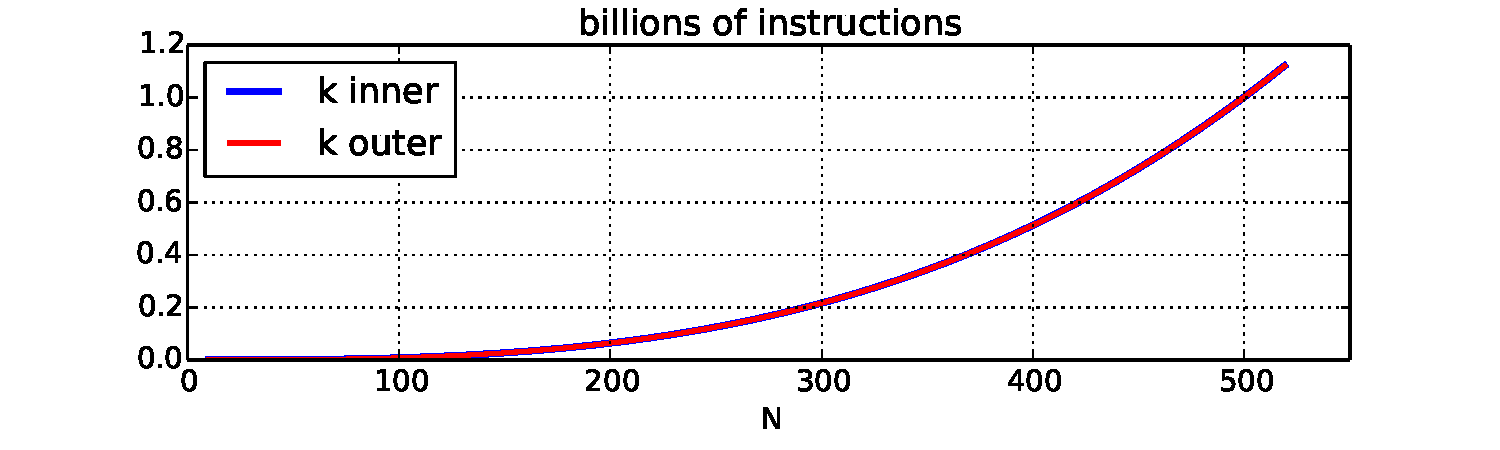
\includegraphics[width=0.99\textwidth]{../caching/k-inout-instrs} \\
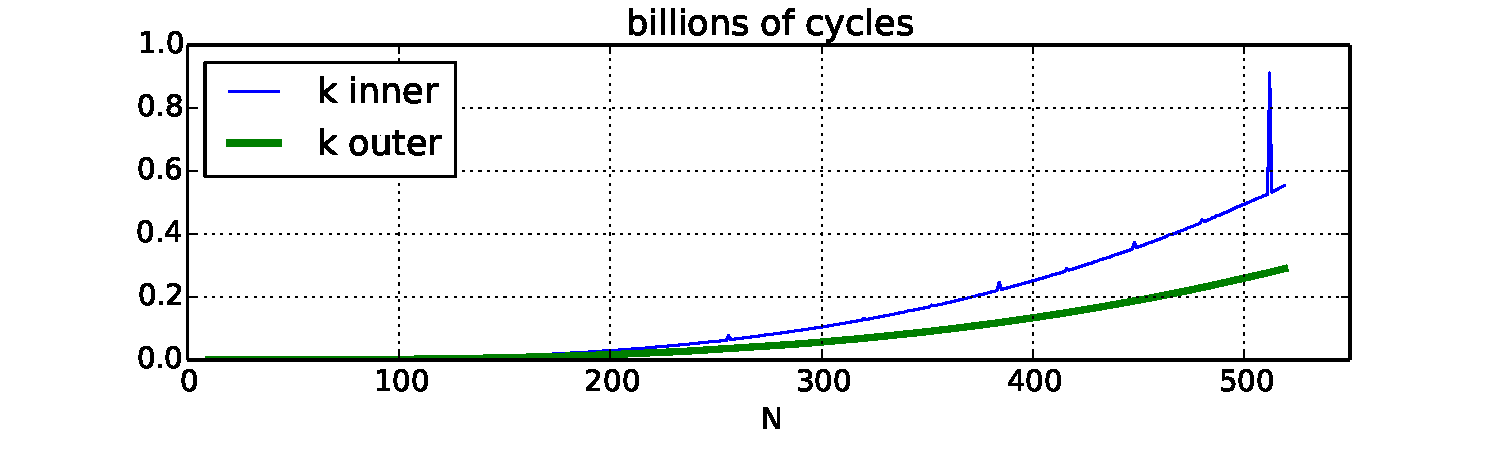
\includegraphics[width=0.99\textwidth]{../caching/k-inout-cycles}
\end{frame}

\begin{frame}{alternate view 1: cycles/instruction}
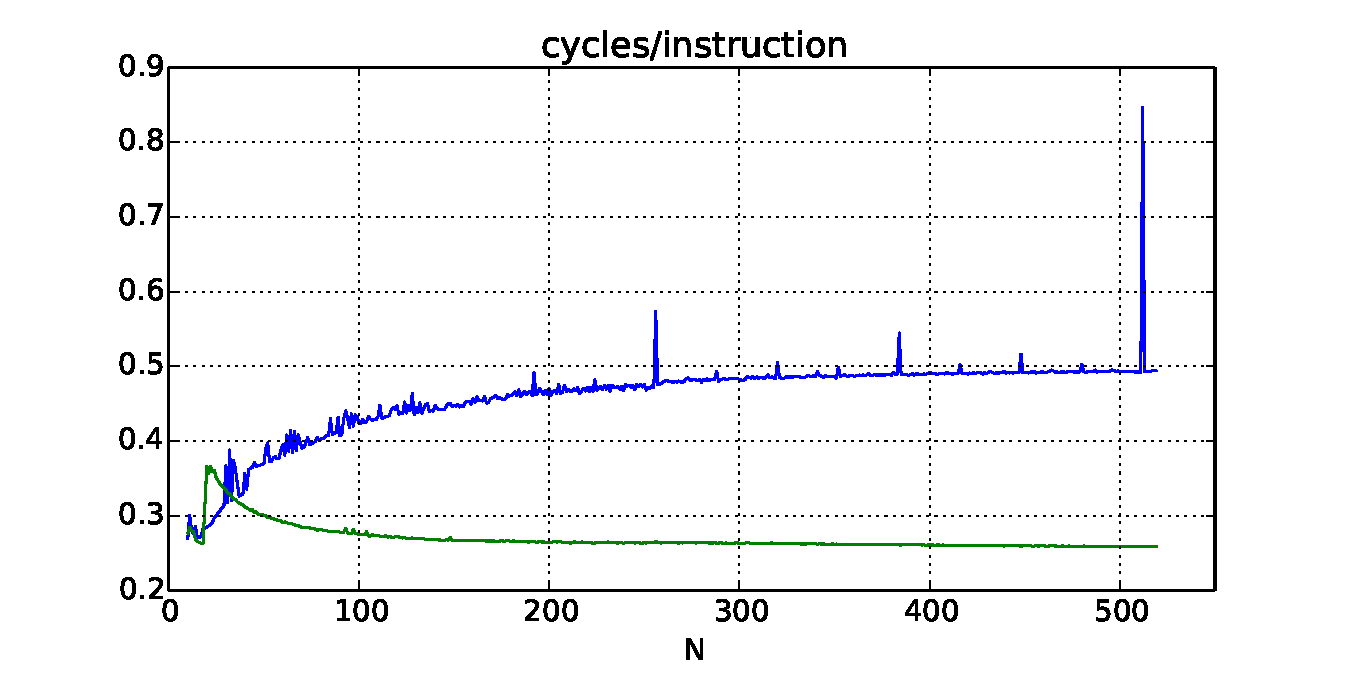
\includegraphics[width=0.99\textwidth]{../caching/k-inout-cpi}
\end{frame}

\begin{frame}{alternate view 2: cycles/operation}
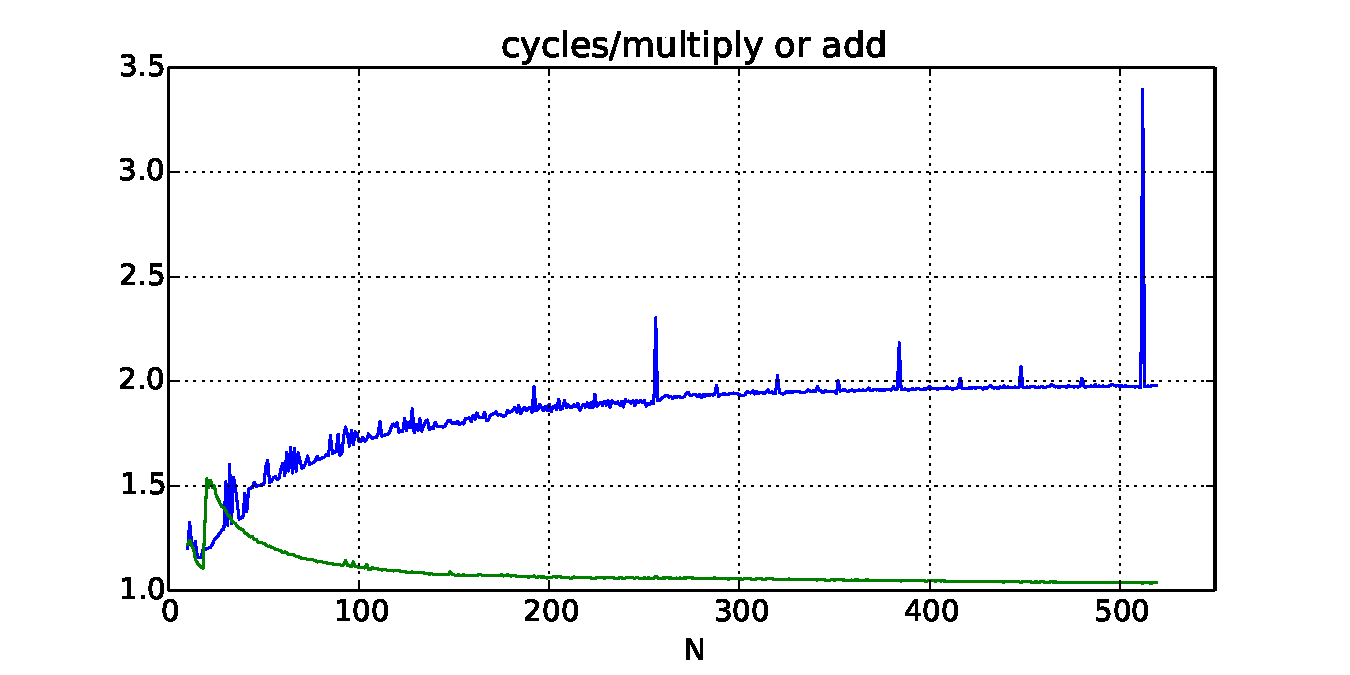
\includegraphics[width=0.99\textwidth]{../caching/k-inout-cpe}
\end{frame}


\subsubsection{miss counting}
\begin{frame}[fragile,label=countingMissesV1]{counting misses: version 1}
\lstset{style=smaller,language=C++}
\begin{lstlisting}
for (int i = 0; i < N; ++i)
  for (int j = 0; j < N; ++j)
    for (int k = 0; k < N; ++k)
      C[i * N + j] += A[i * N + k] * B[k * N + j];
\end{lstlisting}
\begin{itemize}
\item if $N$ really large
    \begin{itemize}
    \item assumption: can't get close to storing $N$ values in cache at once
    \end{itemize}
\item for A: about $N\div \text{block size}$ misses per k-loop
    \begin{itemize}
    \item total misses: $N^3\div\text{block size}$
    \end{itemize}
\item for B: about $N$ misses per k-loop 
    \begin{itemize}
    \item total misses: $N^3$
    \end{itemize}
\item for C: about $1\div\text{block size}$ miss per k-loop
    \begin{itemize}
    \item total misses: $N^2\div\text{block size}$
    \end{itemize}
\end{itemize}
\end{frame}

\begin{frame}[fragile,label=countingMissesV2]{counting misses: version 2}
\lstset{style=smaller,language=C++}
\begin{lstlisting}
for (int k = 0; k < N; ++k)
  for (int i = 0; i < N; ++i)
    for (int j = 0; j < N; ++j)
      C[i * N + j] += A[i * N + k] * B[k * N + j];
\end{lstlisting}
\begin{itemize}
\item for A: about $1$ misses per j-loop
    \begin{itemize}
    \item total misses: $N^2$
    \end{itemize}
\item for B: about $N\div\text{block size}$ miss per j-loop
    \begin{itemize}
    \item total misses: $N^3\div\text{block size}$
    \end{itemize}
\item for C: about $N\div\text{block size}$ miss per j-loop
    \begin{itemize}
    \item total misses: $N^3\div\text{block size}$
    \end{itemize}
\end{itemize}
\end{frame}


\subsubsection{miss count exericse}
\begin{frame}[fragile,label=missEstExer2]{exercise: miss estimating (2)}
\begin{lstlisting}[language=C++,style=small]
for (int k = 0; k < 1000; k += 1)
    for (int i = 0; i < 1000; i += 1)
        for (int j = 0; j < 1000; j += 1)
            A[k*N+j] += B[i*N+j];
\end{lstlisting}
\begin{itemize}
\item assuming: 4 elements per block
\item assuming: cache not close to big enough to hold 1K elements
\vspace{.5cm}
\item estimate: \textit{approximately} how many misses for \textit{A}, \textit{B}?
\end{itemize}
\end{frame}


\subsubsection{jagged edges: conflict misses} % FIXME: cut if not time


\begin{frame}{L1 misses (with A=B)}
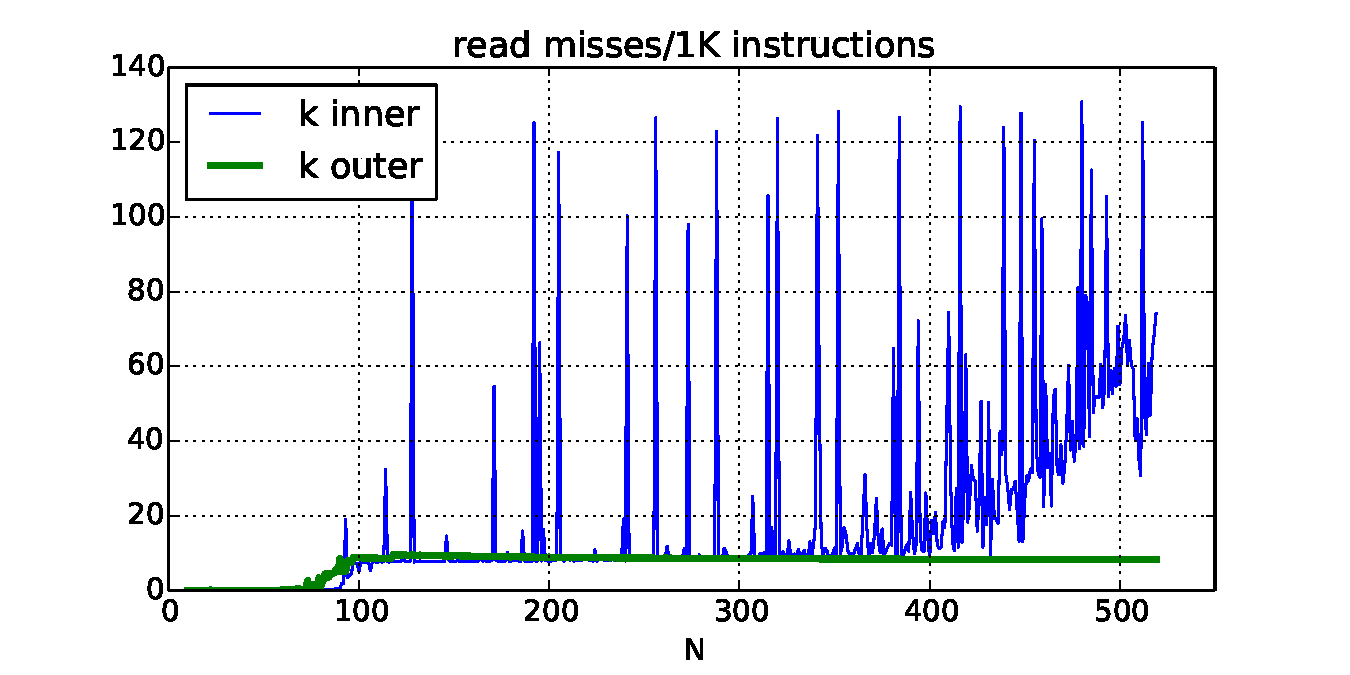
\includegraphics[width=0.99\textwidth]{../caching/k-inout-l1d_read_miss_rate}
\end{frame}

\begin{frame}{L1 miss detail (1)}
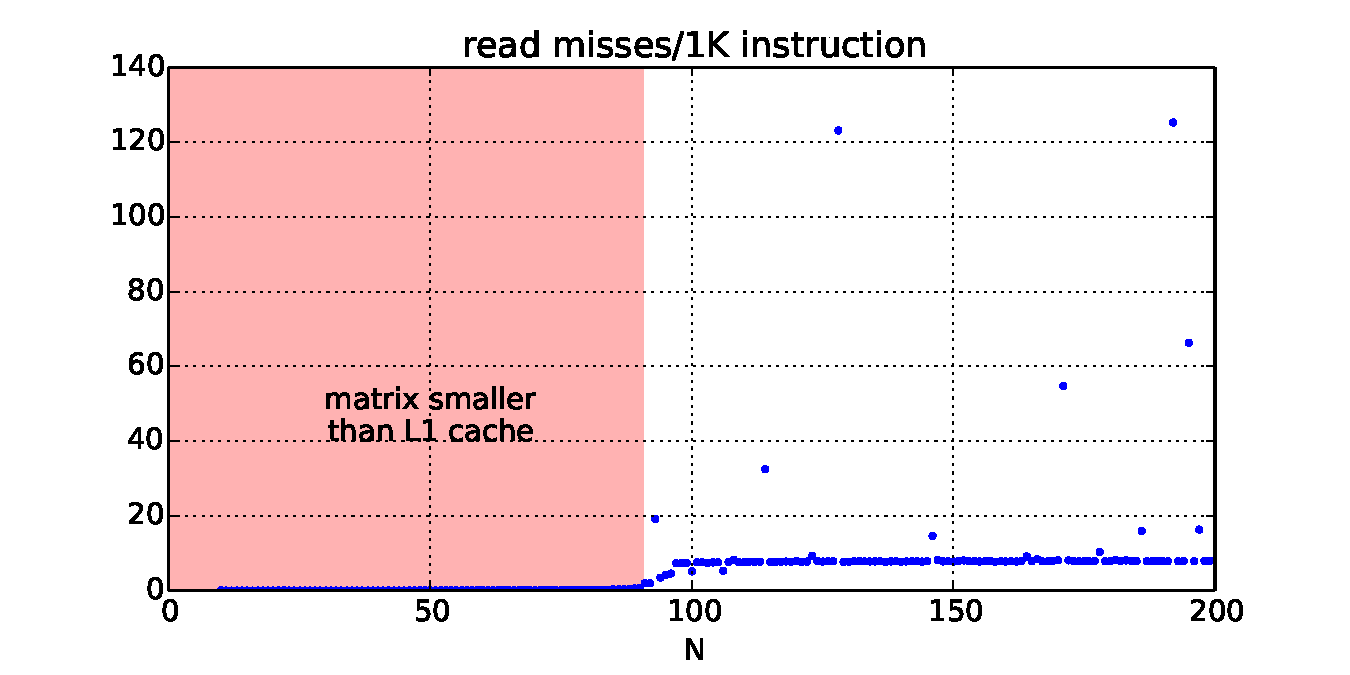
\includegraphics[width=0.99\textwidth]{../caching/k-in-l1d-miss-annot-size}
\end{frame}

\begin{frame}{L1 miss detail (2)}
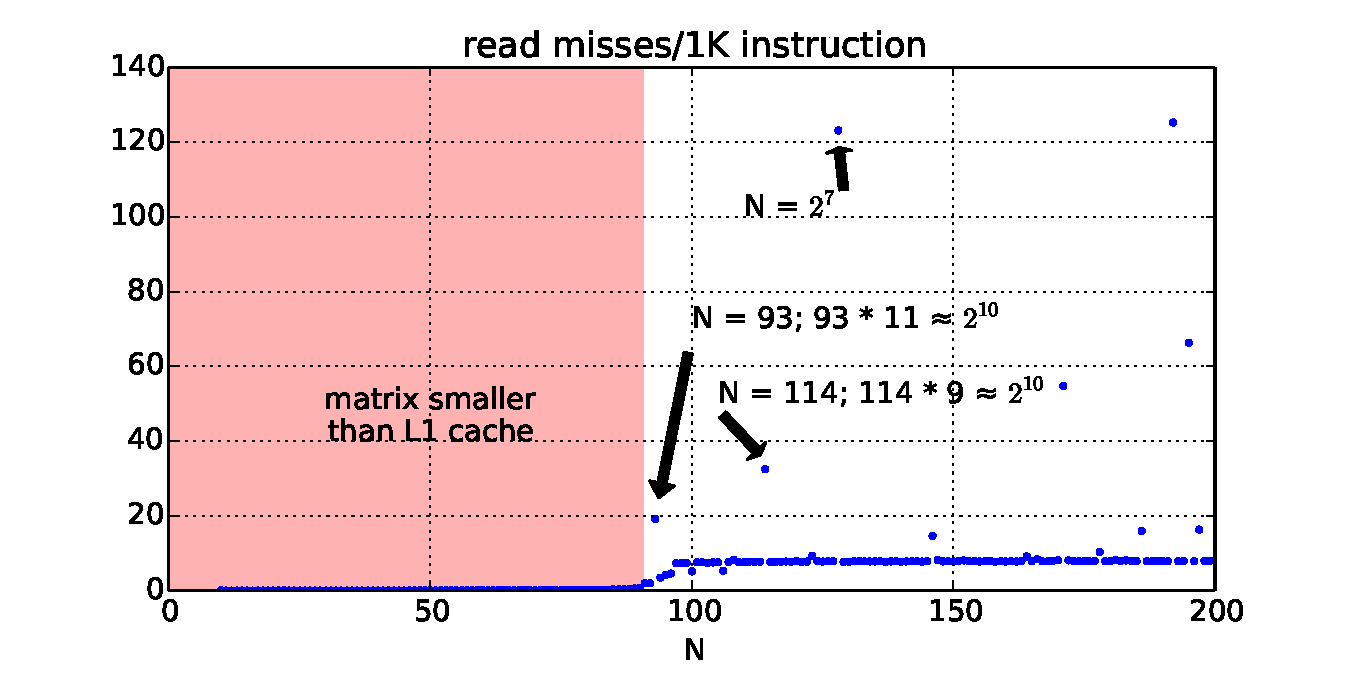
\includegraphics[width=0.99\textwidth]{../caching/k-in-l1d-miss-annot4-size}
\end{frame}

\begin{frame}[fragile,label=conflictExplainPre]{addresses}
    \begin{tabular}{lll}
        \lstinline|B[k*114+j]| &is at& \texttt{10 \textcolor<2>{blue!70!black}{\textbf<2>{0000 00}}00 0100} \\
        \lstinline|B[k*114+j+1]| &is at& \texttt{10 \textcolor<2>{blue!70!black}{\textbf<2>{0000 00}}00 1000} \\
        \lstinline|B[(k+1)*114+j]| &is at& \texttt{10 \textcolor<2>{blue!70!black}{\textbf<2>{0011 10}}01 0100} \\
        \lstinline|B[(k+2)*114+j]| &is at& \texttt{10 \textcolor<2>{blue!70!black}{\textbf<2>{0101 01}}01 1100} \\ 
        \ldots && \\
        \lstinline|B[(k+9)*114+j]| &is at& \texttt{11 \textcolor<2>{blue!70!black}{\textbf<2>{0000 00}}00 1100} \\
    \end{tabular}
    \vspace{.5cm}
    \begin{itemize}
\item<2> test system L1 cache: \textcolor<2>{blue!70!black}{6 index bits}, 6 block offset bits
\end{itemize}

\end{frame}


\begin{frame}[fragile,label=conflictExplain]{conflict misses}
\begin{itemize}
\item powers of two --- lower order bits unchanged
\item \lstinline|B[k*93+j]| and \lstinline|B[(k+11)*93+j]|:
    \begin{itemize}
        \item \myemph{1023 elements apart} (4092 bytes; 63.9 cache blocks)
    \end{itemize}
\item 64 sets in L1 cache: usually maps to same set
\item \lstinline|B[k*93+(j+1)]| will not be cached (next $i$ loop)
\item even if in same block as \lstinline|B[k*93+j]|
\vspace{.5cm}
\item how to fix? improve spatial locality
    \begin{itemize}
    \item (maybe even if it requires copying)
    \end{itemize}
\end{itemize}
\end{frame}



\subsection{warmup, take two: locality exercise}

\begin{frame}[fragile,label=localityExercise2]{locality exercise (2)}
\lstset{language=C,style=small}
\begin{lstlisting}
/* version 2 */
for (int i = 0; i < N; ++i)
    for (int j = 0; j < N; ++j)
        A[i] += B[j] * C[i * N + j]

/* version 3 */
for (int ii = 0; ii < N; ii += 32)
    for (int jj = 0; jj < N; jj += 32)
        for (int i = ii; i < ii + 32; ++i)
            for (int j = jj; j < jj + 32; ++j)
                A[i] += B[j] * C[i * N + j];
\end{lstlisting}
exercise: which has better temporal locality in A? in B? in C? \\
how about spatial locality?
\end{frame}



\subsection{cache blocking introduction}
%\begin{frame}[fragile,label=cacheBlockKPrep]{a transformation}
\lstset{
    style=small,language=C,escapechar=@,
    moredelim=**[is][\btHL<2>]{~2}{~},
    moredelim=**[is][\btHL<3>]{~3}{~},
    moredelim=**[is][\btHL<4>]{~4}{~},
}
\begin{lstlisting}
for (int kk = 0; kk < N; ~2kk += 2~)
  for (int k = kk; ~2k < kk + 2~; ++k)
      for (int i = 0; i < N; ++i)
        for (int j = 0; j < N; ++j)
          B[i*N+j] += A[i*N+k] * A[k*N+j];
\end{lstlisting}
\begin{itemize}
\item split the loop over $k$ --- should be exactly the same 
    \begin{itemize}
    \item (assuming even $N$)
    \end{itemize}
\end{itemize}
\end{frame}

\begin{frame}[fragile,label=cacheBlockK]{simple blocking}
\lstset{
    style=small,language=C,escapechar=@,
    moredelim=**[is][\btHL<2>]{~2}{~},
    moredelim=**[is][\btHL<2-3>]{~3}{~},
    moredelim=**[is][\btHL<4>]{~4}{~},
}
\begin{lstlisting}
for (int kk = 0; kk < N; ~2kk += 2~)
  /* was here: for (int k = kk; k < kk + 2; ++k) */
    for (int i = 0; i < N; ++i)
      for (int j = 0; j < N; ++j)
        /* load Aik, Aik+1 into cache and process: */
        ~3for (int k = kk; k < kk + 2; ++k)~
            B[i*N+j] += A[i*N+k] * A[k*N+j];
\end{lstlisting}
\begin{itemize}
\item now \myemph{reorder} split loop --- same calculations
\item<2-> now handle $B_{ij}$ for $k+1$ right after $B_{ij}$ for $k$
\item<2-> (previously: $B_{i,j+1}$ for $k$ right after $B_{ij}$ for $k$)
\end{itemize}
\end{frame}

\begin{frame}[fragile,label=cacheBlockKExpand]{simple blocking -- expanded}
\lstset{
    style=small,language=C,escapechar=@,
    moredelim=**[is][\btHL<2>]{~2}{~},
    moredelim=**[is][\btHL<3>]{~3}{~},
    moredelim=**[is][\btHL<4>]{~4}{~},
}
\begin{lstlisting}
for (int kk = 0; kk < N; kk += 2) {
  for (int i = 0; i < N; i += 2) {
    for (int j = 0; j < N; ++j) {
      /* process a "block" of 2 k values: */
      ~2B[i*N+j]~ += ~3A[i*N+kk+0]~ * ~4A[(kk+0)*N+j]~;
      ~2B[i*N+j]~ += ~3A[i*N+kk+1]~ * A[(kk+1)*N+j];
    }
  }
}
\end{lstlisting}
\begin{itemize}
\item \only<2>{Temporal locality in $B_{ij}$s}
      \only<3>{More spatial locality in $A_{ik}$}
      \only<4>{Still have good spatial locality in $A_{kj}$, $B_{ij}$}
\end{itemize}
\end{frame}

\begin{frame}{improvement in read misses}
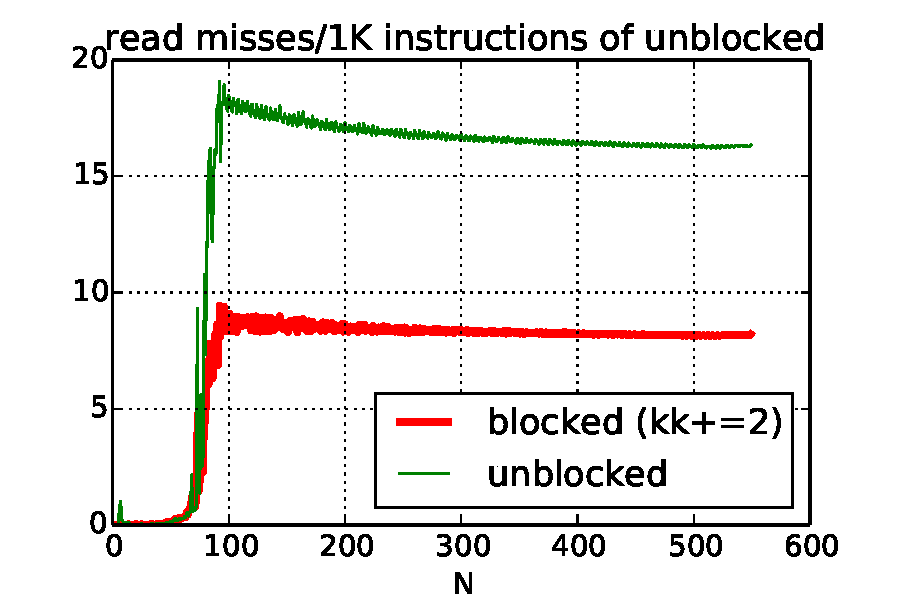
\includegraphics[width=0.8\textwidth]{../caching/k-kk-novec-block-read_miss_rate}
\end{frame}


\begin{frame}[fragile,label=cacheBlockExamplePartial]{simple blocking (2)}
\lstset{
    style=small,language=C,escapechar=@,
    moredelim=**[is][\btHL<2>]{~2}{~},
    moredelim=**[is][\btHL<3>]{~3}{~},
    moredelim=**[is][\btHL<4>]{~4}{~},
}
\begin{itemize}
\item same thing for $i$ in addition to $k$?
\end{itemize}
\begin{lstlisting}
for (int kk = 0; kk < N; kk += 2) {
  for (int ii = 0; ii < N; ii += 2) {
    for (int j = 0; j < N; ++j) {
      /* process a "block": */
      for (int k = kk; k < kk + 2; ++k)
        for (int i = 0; i < ii + 2; ++i)
            B[i*N+j] += A[i*N+k] * A[k*N+j];
    }
  }
}
\end{lstlisting}
\end{frame}

\begin{frame}[fragile,label=cacheBlockExamplePartialExpand]{simple blocking --- expanded}
\lstset{style=small,language=C,escapechar=@}
\begin{lstlisting}
for (int k = 0; k < N; k += 2) {
  for (int i = 0; i < N; i += 2) {
    /* load a block around Aik */
    for (int j = 0; j < N; ++j) {
      /* process a "block": */
      @\normalsize$B_{i+0,j}$@ += @\normalsize$A_{i+0,k+0}$@ * @\normalsize\myemph{$A_{k+0,j}$}@
      @\normalsize$B_{i+0,j}$@ += @\normalsize$A_{i+0,k+1}$@ * @\normalsize$A_{k+1,j}$@
      @\normalsize$B_{i+1,j}$@ += @\normalsize$A_{i+1,k+0}$@ * @\normalsize\myemph{$A_{k+0,j}$}@
      @\normalsize$B_{i+1,j}$@ += @\normalsize$A_{i+1,k+1}$@ * @\normalsize$A_{k+1,j}$@
    }
  }
}
\end{lstlisting}
\begin{itemize}
\item<2-> Now $A_{kj}$ reused in inner loop --- more calculations per load!
\end{itemize}
\end{frame}


\subsubsection{transformation --- 1D blocking}
\begin{frame}[fragile,label=cacheBlockKPrep]{a transformation}
\lstset{
    style=small,language=C,escapechar=@,
    moredelim=**[is][\btHL<2>]{~2}{~},
    moredelim=**[is][\btHL<3>]{~3}{~},
    moredelim=**[is][\btHL<4>]{~4}{~},
}
\begin{lstlisting}
for (int k = 0; k < N; ~2k += 1~)
      for (int i = 0; i < N; ++i)
        for (int j = 0; j < N; ++j)
          C[i*N+j] += A[i*N+k] * B[k*N+j];
\end{lstlisting}
\hrule
\begin{lstlisting}
for (int kk = 0; kk < N; ~2kk += 2~)
  for (int k = kk; ~2k < kk + 2~; ++k)
      for (int i = 0; i < N; ++i)
        for (int j = 0; j < N; ++j)
          C[i*N+j] += A[i*N+k] * B[k*N+j];
\end{lstlisting}
\begin{itemize}
\item split the loop over $k$ --- should be exactly the same 
    \begin{itemize}
    \item (assuming even $N$)
    \end{itemize}
\end{itemize}
\end{frame}

\begin{frame}[fragile,label=cacheBlockK]{simple blocking}
\lstset{
    style=small,language=C,escapechar=@,
    moredelim=**[is][\btHL<2>]{~2}{~},
    moredelim=**[is][\btHL<2-3>]{~3}{~},
    moredelim=**[is][\btHL<4>]{~4}{~},
}
\begin{lstlisting}
for (int kk = 0; kk < N; ~2kk += 2~)
  /* was here: for (int k = kk; k < kk + 2; ++k) */
    for (int i = 0; i < N; ++i)
      for (int j = 0; j < N; ++j)
        /* load Aik, Aik+1 into cache and process: */
        ~3for (int k = kk; k < kk + 2; ++k)~
            C[i*N+j] += A[i*N+k] * B[k*N+j];
\end{lstlisting}
\begin{itemize}
\item now \myemph{reorder} split loop --- same calculations
\item<2-> now handle $B_{ij}$ for $k+1$ right after $B_{ij}$ for $k$
\item<2-> (previously: $B_{i,j+1}$ for $k$ right after $B_{ij}$ for $k$)
\end{itemize}
\end{frame}

\begin{frame}[fragile,label=cacheBlockKExpand]{simple blocking -- expanded}
\lstset{
    style=small,language=C,escapechar=@,
    moredelim=**[is][\btHL<2>]{~2}{~},
    moredelim=**[is][\btHL<3>]{~3}{~},
    moredelim=**[is][\btHL<4>]{~4}{~},
}
\begin{lstlisting}
for (int kk = 0; kk < N; kk += 2) {
  for (int i = 0; i < N; ++i) {
    for (int j = 0; j < N; ++j) {
      /* process a "block" of 2 k values: */
      ~2C[i*N+j]~ += ~3A[i*N+kk+0]~ * ~4B[(kk+0)*N+j]~;
      ~2C[i*N+j]~ += ~3A[i*N+kk+1]~ * B[(kk+1)*N+j];
    }
  }
}
\end{lstlisting}
\begin{itemize}
\item \only<2>{Temporal locality in $C_{ij}$s}
      \only<3>{More spatial locality in $A_{ik}$}
      \only<4>{Still have good spatial locality in $B_{kj}$, $C_{ij}$}
\end{itemize}
\end{frame}


%\subsubsection{missses in A}

\begin{frame}[fragile,label=cacheBlockKLoadsA]{counting misses for A (1)}
\lstset{
    style=smaller,language=C,escapechar=@,
    moredelim=**[is][\btHL<0>]{~2}{~},
    moredelim=**[is][\btHL<0>]{~3}{~},
    moredelim=**[is][\btHL<0>]{~4}{~},
}
\begin{lstlisting}
for (int kk = 0; kk < N; kk += 2)
  for (int i = 0; i < N; i += 1)
    for (int j = 0; j < N; ++j) {
      ~2C[i*N+j]~ += ~3A[i*N+kk+0]~ * ~4B[(kk+0)*N+j]~;
      ~2C[i*N+j]~ += ~3A[i*N+kk+1]~ * ~4B[(kk+1)*N+j]~;
    }
\end{lstlisting}
access pattern for A: \\
\myemph<2-3>{A[0*N+0], A[0*N+1]}, A[0*N+0], A[0*N+1] \ldots (repeats N times) \\
\myemph<2-3>{A[1*N+0], A[1*N+1]}, A[1*N+0], A[1*N+1] \ldots (repeats N times) \\
\ldots \\
\only<2->{A[(N-1)*N+0], A[(N-1)*N+1], A[(N-1)*N+0], A[(N-1)*N+1] \ldots} \\
\only<2->{A[0*N+2], A[0*N+3], A[0*N+2], A[0*N+3] \ldots} \\
\ldots 
\end{frame}

\begin{frame}[fragile,label=cacheBlockKLoadsA2]{counting misses for A (2)}
\myemph<2-3>{A[0*N+0], A[0*N+1]}, A[0*N+0], A[0*N+1] \ldots (repeats N times) \\
\myemph<2-3>{A[1*N+0], A[1*N+1]}, A[1*N+0], A[1*N+1] \ldots (repeats N times) \\
\ldots \\
\only<2->{\myemph<2-3>{A[(N-1)*N+0], A[(N-1)*N+1]}, A[(N-1)*N+0], A[(N-1)*N+1] \ldots} \\
\only<2->{\myemph<2-3>{A[0*N+2], A[0*N+3]}, A[0*N+2], A[0*N+3] \ldots} \\
\ldots 
\begin{itemize}
\item<2-> likely cache misses: only first iterations of $j$ loop
\item<2-> how many cache misses per iteration? usually one
    \begin{itemize}
    \item A[0*N+0] and A[0*N+1] usually in same cache block
    \end{itemize}
\item<3-> about $\frac{N}{2}\cdot N$ misses total
\end{itemize}
\end{frame}

%\subsubsection{missses in B}
\begin{frame}[fragile,label=cacheBlockKLoadsB]{counting misses for B (1)}
\lstset{
    style=small,language=C,escapechar=@,
    moredelim=**[is][\btHL<0>]{~2}{~},
    moredelim=**[is][\btHL<0>]{~3}{~},
    moredelim=**[is][\btHL<0>]{~4}{~},
}
\begin{lstlisting}
for (int kk = 0; kk < N; kk += 2)
  for (int i = 0; i < N; i += 1)
    for (int j = 0; j < N; ++j) {
      ~2C[i*N+j]~ += ~3A[i*N+kk+0]~ * ~4B[(kk+0)*N+j]~;
      ~2C[i*N+j]~ += ~3A[i*N+kk+1]~ * ~4B[(kk+1)*N+j]~;
    }
\end{lstlisting}
access pattern for B: \\
B[0*N+0], B[1*N+0], \ldots B[0*N+(N-1)], B[1*N+(N-1)] \\
B[2*N+0], B[3*N+0], \ldots B[2*N+(N-1)], B[3*N+(N-1)] \\
B[4*N+0], B[5*N+0], \ldots B[4*N+(N-1)], B[5*N+(N-1)] \\
\ldots \\
B[0*N+0], B[1*N+0], \ldots B[0*N+(N-1)], B[1*N+(N-1)] \\
\ldots
\end{frame}

\begin{frame}{counting misses for B (2)}
access pattern for B: \\
B[0*N+0], B[1*N+0], \ldots B[0*N+(N-1)], B[1*N+(N-1)] \\
B[2*N+0], B[3*N+0], \ldots B[2*N+(N-1)], B[3*N+(N-1)] \\
B[4*N+0], B[5*N+0], \ldots B[4*N+(N-1)], B[5*N+(N-1)] \\
\ldots \\
B[0*N+0], B[1*N+0], \ldots B[0*N+(N-1)], B[1*N+(N-1)] \\
\ldots
\begin{itemize}
\item<2-> likely cache misses: any access, each time
\item<3-> how many cache misses per iteration? equal to \# cache blocks in 2 rows
\item<4-> about $\frac{N}{2}\cdot N\cdot\frac{2N}{\text{block size}}=N^3\div\text{block size}$ misses
\end{itemize}
\end{frame}



%\subsubsection{overall misses}
\begin{frame}[fragile,label=cacheBlockKLoads]{simple blocking -- counting misses}
\lstset{
    style=smaller,language=C,escapechar=@,
    moredelim=**[is][\btHL<0>]{~2}{~},
    moredelim=**[is][\btHL<0>]{~3}{~},
    moredelim=**[is][\btHL<0>]{~4}{~},
}
\begin{lstlisting}
for (int kk = 0; kk < N; kk += 2)
  for (int i = 0; i < N; i += 1)
    for (int j = 0; j < N; ++j) {
      ~2C[i*N+j]~ += ~3A[i*N+kk+0]~ * ~4B[(kk+0)*N+j]~;
      ~2C[i*N+j]~ += ~3A[i*N+kk+1]~ * ~4B[(kk+1)*N+j]~;
    }
\end{lstlisting}
\begin{itemize}
\item $\frac{N}{2}\cdot N$ j-loop executions and (assuming $N$ large):
\item about $1$ misses from $A$ per j-loop 
    \begin{itemize}
    \item \myemph<2>{$N^2/2$ total misses (before blocking: $N^2$)}
    \end{itemize}
\item about $2N\div\text{block size}$ misses from $B$ per j-loop 
    \begin{itemize}
    \item $N^3\div\text{block size}$ total misses (same as before blocking)
    \end{itemize}
\item about $N\div\text{block size}$ misses from $C$ per j-loop 
    \begin{itemize}
    \item \myemph<2>{$N^3\div(2\cdot\text{block size})$ total misses (before: $N^3\div\text{block size}$)}
    \end{itemize}
\end{itemize}
\end{frame}


%\subsubsection{actual performance}

\begin{frame}{improvement in read misses}
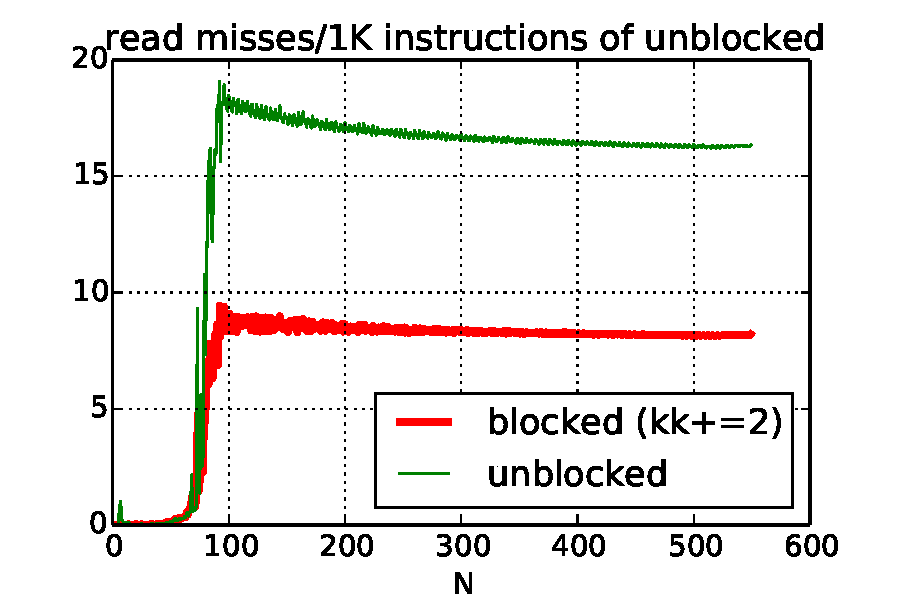
\includegraphics[width=0.8\textwidth]{../caching/k-kk-novec-block-read_miss_rate}
\end{frame}



\subsubsection{two-at-a-time}


\begin{frame}[fragile,label=cacheBlockExamplePartial]{simple blocking (2)}
\lstset{
    style=small,language=C,escapechar=@,
    moredelim=**[is][\btHL<2>]{~2}{~},
    moredelim=**[is][\btHL<3>]{~3}{~},
    moredelim=**[is][\btHL<4>]{~4}{~},
}
\begin{itemize}
\item same thing for $i$ in addition to $k$?
\end{itemize}
\begin{lstlisting}
for (int kk = 0; kk < N; kk += 2) {
  for (int ii = 0; ii < N; ii += 2) {
    for (int j = 0; j < N; ++j) {
      /* process a "block": */
      for (int k = kk; k < kk + 2; ++k)
        for (int i = 0; i < ii + 2; ++i)
            C[i*N+j] += A[i*N+k] * B[k*N+j];
    }
  }
}
\end{lstlisting}
\end{frame}

\begin{frame}[fragile,label=cacheBlockExamplePartialExpand]{simple blocking --- locality}
\lstset{style=smaller,language=C,escapechar=@}
\begin{lstlisting}
for (int k = 0; k < N; k += 2) {
  for (int i = 0; i < N; i += 2) {
    /* load a block around Aik */
    for (int j = 0; j < N; ++j) {
      /* process a "block": */
      @\normalsize$C_{i+0,j}$@ += @\normalsize$A_{i+0,k+0}$@ * @\normalsize\myemph{$B_{k+0,j}$}@
      @\normalsize$C_{i+0,j}$@ += @\normalsize$A_{i+0,k+1}$@ * @\normalsize$B_{k+1,j}$@
      @\normalsize$C_{i+1,j}$@ += @\normalsize$A_{i+1,k+0}$@ * @\normalsize\myemph{$B_{k+0,j}$}@
      @\normalsize$C_{i+1,j}$@ += @\normalsize$A_{i+1,k+1}$@ * @\normalsize$B_{k+1,j}$@
    }
  }
}
\end{lstlisting}
\begin{itemize}
\item<2-> now: more temporal locality in $B$
    \begin{itemize}
    \item previously: access $B_{kj}$, then don't use it again for a \myemph{long} time
    \end{itemize}
\end{itemize}
\end{frame}

\begin{frame}[fragile,label=cacheBlockExamplePartialMissesA]{simple blocking --- counting misses for A}
\lstset{style=small,language=C,escapechar=@}
\begin{lstlisting}
for (int k = 0; k < N; k += 2)
  for (int i = 0; i < N; i += 2)
    for (int j = 0; j < N; ++j) {
      @\normalsize$C_{i+0,j}$@ += @\normalsize$A_{i+0,k+0}$@ * @\normalsize$B_{k+0,j}$@
      @\normalsize$C_{i+0,j}$@ += @\normalsize$A_{i+0,k+1}$@ * @\normalsize$B_{k+1,j}$@
      @\normalsize$C_{i+1,j}$@ += @\normalsize$A_{i+1,k+0}$@ * @\normalsize$B_{k+0,j}$@
      @\normalsize$C_{i+1,j}$@ += @\normalsize$A_{i+1,k+1}$@ * @\normalsize$B_{k+1,j}$@
    }
\end{lstlisting}
\begin{itemize}
\item $\frac{N}{2}\cdot\frac{N}{2}$ iterations of $j$ loop
\item likely 2 misses per loop with $A$ (2 cache blocks)
    \begin{itemize}
    \item total misses: $\frac{N^2}{2}$ (same as only blocking in K)
    \end{itemize}
\end{itemize}
\end{frame}

\begin{frame}[fragile,label=cacheBlockExamplePartialMissesB]{simple blocking --- counting misses for B}
\lstset{style=small,language=C,escapechar=@}
\begin{lstlisting}
for (int k = 0; k < N; k += 2)
  for (int i = 0; i < N; i += 2)
    for (int j = 0; j < N; ++j) {
      @\normalsize$C_{i+0,j}$@ += @\normalsize$A_{i+0,k+0}$@ * @\normalsize\myemph{$B_{k+0,j}$}@
      @\normalsize$C_{i+0,j}$@ += @\normalsize$A_{i+0,k+1}$@ * @\normalsize$B_{k+1,j}$@
      @\normalsize$C_{i+1,j}$@ += @\normalsize$A_{i+1,k+0}$@ * @\normalsize\myemph{$B_{k+0,j}$}@
      @\normalsize$C_{i+1,j}$@ += @\normalsize$A_{i+1,k+1}$@ * @\normalsize$B_{k+1,j}$@
    }
\end{lstlisting}
\begin{itemize}
\item $\frac{N}{2}\cdot\frac{N}{2}$ iterations of $j$ loop
\item likely $2\div\text{block size}$ misses per iteration with $B$
    \begin{itemize}
    \item total misses: $\frac{N^3}{2\cdot\text{block size}}$ (before: $\frac{N^3}{\text{block size}}$)
    \end{itemize}
\end{itemize}
\end{frame}

\begin{frame}[fragile,label=cacheBlockExamplePartialMissesC]{simple blocking --- counting misses for C}
\lstset{style=small,language=C,escapechar=@}
\begin{lstlisting}
for (int k = 0; k < N; k += 2)
  for (int i = 0; i < N; i += 2)
    for (int j = 0; j < N; ++j) {
      @\normalsize$C_{i+0,j}$@ += @\normalsize$A_{i+0,k+0}$@ * @\normalsize{$B_{k+0,j}$}@
      @\normalsize$C_{i+0,j}$@ += @\normalsize$A_{i+0,k+1}$@ * @\normalsize$B_{k+1,j}$@
      @\normalsize$C_{i+1,j}$@ += @\normalsize$A_{i+1,k+0}$@ * @\normalsize{$B_{k+0,j}$}@
      @\normalsize$C_{i+1,j}$@ += @\normalsize$A_{i+1,k+1}$@ * @\normalsize$B_{k+1,j}$@
    }
\end{lstlisting}
\begin{itemize}
\item $\frac{N}{2}\cdot\frac{N}{2}$ iterations of $j$ loop
\item likely $\frac{2}{\text{block size}}$ misses per iteration with $C$
    \begin{itemize}
    \item total misses: $\frac{N^3}{2\cdot\text{block size}}$ (same as blocking only in K)
    \end{itemize}
\end{itemize}
\end{frame}

\begin{frame}[fragile,label=cacheBlockExamplePartialMissesTot]{simple blocking --- counting misses (total)}
\lstset{style=small,language=C,escapechar=@}
\begin{lstlisting}
for (int k = 0; k < N; k += 2)
  for (int i = 0; i < N; i += 2)
    for (int j = 0; j < N; ++j) {
      @\normalsize$C_{i+0,j}$@ += @\normalsize$A_{i+0,k+0}$@ * @\normalsize{$B_{k+0,j}$}@
      @\normalsize$C_{i+0,j}$@ += @\normalsize$A_{i+0,k+1}$@ * @\normalsize$B_{k+1,j}$@
      @\normalsize$C_{i+1,j}$@ += @\normalsize$A_{i+1,k+0}$@ * @\normalsize{$B_{k+0,j}$}@
      @\normalsize$C_{i+1,j}$@ += @\normalsize$A_{i+1,k+1}$@ * @\normalsize$B_{k+1,j}$@
    }
\end{lstlisting}
\begin{itemize}
\item before: \\
A: $\frac{N^2}{2}$; B: $\frac{N^3}{1\cdot\text{block size}}$; C $\frac{N^3}{1\cdot\text{block size}}$
\item after: \\
A: $\frac{N^2}{2}$; B: $\frac{N^3}{2\cdot\text{block size}}$; C $\frac{N^3}{2\cdot\text{block size}}$
\end{itemize}
\end{frame}

%\begin{frame}[fragile,label=cacheBlockExample]{generalizing cache blocking}
\lstset{
    style=smaller,language=C,escapechar=@,
    moredelim=**[is][\btHL<all:2>]{~2}{~},
    moredelim=**[is][\btHL<all:3>]{~3}{~},
    moredelim=**[is][\btHL<all:4>]{~4}{~},
}
\vspace{-.25cm}
\begin{lstlisting}
for (int kk = 0; kk < N; kk += K) {
  for (int ii = 0; ii < N; ii += I) {
    @\sffamily with I by K block of A hopefully cached:@
    for (int jj = 0; jj < N; jj += J) {
      @\sffamily with K by J block of A, I by J block of B cached:@
      for i in ii to ii+I:
        for j in jj to jj+J:
          for k in kk to kk+K:
            ~2B[i * N + j]~ += ~3A[i * N + k]~
                          * ~4A[k * N + j]~;
\end{lstlisting}
\begin{itemize}
    \item \myemph<2>{$B_{ij}$} used $K$ times for one miss --- $N^2/K$ misses
    \item \myemph<3>{$A_{ik}$} used $J$ times for one miss --- $N^2/J$ misses
    \item \myemph<4>{$A_{kj}$} used $I$ times for one miss --- $N^2/I$ misses
\item catch: $IK+KJ+IJ$ elements must \myemph{fit in cache}
\end{itemize}
\end{frame}

% FIXME: diagram
%
\begin{frame}[fragile,label=cacheDivideConquer]{view 2: divide and conquer}
\lstset{style=small}
\begin{lstlisting}
partial_square(float *A, float *B,
               int startI, int endI, ...) {
  for (int i = startI; i < endI; ++i) {
    for (int j = startJ; j < endJ; ++j) {
      ...
}
square(float *A, float *B, int N) {
  for (int ii = 0; ii < N; ii += BLOCK)
    ...
      /* segment of A, B in use fits in cache! */
      partial_square(
            A, B,
            ii, ii + BLOCK,
            jj, jj + BLOCK, ...);
}
\end{lstlisting}
\end{frame}
 % FIXME: earlier?

\subsubsection{generalizing}
\begin{frame}[fragile,label=cacheDivideConquer]{generalizing: divide and conquer}
\lstset{style=small}
\begin{lstlisting}
partial_matrixmultiply(float *A, float *B, float *C
               int startI, int endI, ...) {
  for (int i = startI; i < endI; ++i) {
    for (int j = startJ; j < endJ; ++j) {
      for (int k = startK; k < endK; ++k) {
        ...
}
matrix_multiply(float *A, float *B, float *C, int N) {
  for (int ii = 0; ii < N; ii += BLOCK_I)
    for (int jj = 0; jj < N; jj += BLOCK_J)
      for (int kk = 0; kk < N; kk += BLOCK_K)
         ...
         /* do everything for segment of A, B, C
            that fits in cache! */
         partial_matmul(A, B, C,
               ii, ii + BLOCK_I, jj, jj + BLOCK_J,
               kk, kk + BLOCK_K)
}
\end{lstlisting}
\end{frame}


\subsubsection{diagram of general}
\begin{frame}[fragile,label=cacheBlockBlock]{array usage: matrix block}
\begin{tikzpicture}
\draw[fill=yellow!10] (0, 0) rectangle (4, 4);
\draw[fill=yellow!10] (5, 0) rectangle (9, 4);
\draw[fill=yellow!10] (10, 0) rectangle ++(4, 4);
%\fill[green] (0.5, 1.0) rectangle (1.0, 1.5) node[black,midway,left,fill=none,align=left] {$A_{ik}$ block\\($I\times K$)};
\fill[green] (1.0, 0.5) rectangle ++(0.5, 0.5) node[black,midway,left,fill=none,align=left] {$A_{ik}$ block\\($I\times K$)};
%\fill[green] (1.0, 3.0) rectangle (1.5, 3.5) node[black,midway,above,align=center,fill=none] {$A_{kj}$ block\\($K\times J$)};
\fill[green] (5.+3.0, 3.0) rectangle ++(0.5, 0.5) node[black,midway,above,align=center,fill=none] {$B_{kj}$ block\\($K\times J$)};
%\fill[green] (5.5, 3.0) rectangle (6.0, 3.5) node[black,midway,above,align=center,fill=none] {$B_{ij}$ block\\($I\times J$)};
\fill[green] (5.+8.0, 0.5) rectangle ++(0.5, 0.5) node[black,midway,above,align=center,fill=none] {$C_{ij}$ block\\($I\times J$)};
\begin{visibleenv}<1>
\node[anchor=north,align=left] at (7.5,-1) {
    inner loops work on ``matrix block'' of A, B, C \\
    rather than rows of some, little blocks of others \\
    blocks fit into cache (b/c we choose $I$, $K$, $J$) \\
    where previous rows might not
};
\end{visibleenv}
\begin{visibleenv}<2>
\node[anchor=north,align=left] at (7.5,-1) {
    now (versus loop ordering example) \\
    some spatial locality in A, B, and C \\
    some temporal locality in A, B, and C 
};
\end{visibleenv}
\begin{visibleenv}<3>
%\fill[orange] (0.7,1.0) rectangle (0.8,1.5);
\fill[orange] (1.0,0.7) rectangle (1.5,0.8);
%\fill[orange] (1.0,3.1) rectangle (1.5,3.2);
\fill[orange] (5.+3.1,3.0) rectangle (5.+3.2,3.5);
%\fill[red] (5.7,3.1) rectangle (5.8,3.2);
\fill[red] (5.+8.1,0.7) rectangle (5.+8.2,0.8);
\node[anchor=north,align=left] at (7.5,-1) {
    $C_{ij}$ calculation uses strips from $A$, $B$ \\
    $K$ calculations for one cache miss \\
    good temporal locality!
};
\end{visibleenv}
\begin{visibleenv}<4>
%\fill[red] (0.7,1.1) rectangle (0.8,1.2);
\fill[red] (1.1,0.7) rectangle (1.2,0.8);
%\fill[orange] (1.1,3.0) rectangle (1.2,3.5);
\fill[orange] (5.+3.0,3.1) rectangle (5.+3.5,3.2);
%\fill[orange] (5.7,3.0) rectangle (5.8,3.5);
\fill[orange] (5.+8.0,0.7) rectangle (5.+8.5,0.8);
\node[anchor=north,align=left] at (7.5,-1) {
    $A_{ik}$ used with entire strip of $B$
    $J$ calculations for one cache miss  \\
    good temporal locality!
};
\end{visibleenv}
\begin{visibleenv}<5->
\node[anchor=north,align=left] at (7.5,-0.5) {
    (approx.) $KIJ$ fully cached calculations \\
    for $KI+IJ+KJ$ values need to be lodaed per ``matrix block'' \\
    (assuming everything stays in cache)
};
\end{visibleenv}
\begin{scope}[overlay]
\node[anchor=south west,font=\bfseries] at (7, 4.75) {
    $\mathbf{C_{ij}}$ += $\mathbf{A_{ik}} \cdot \mathbf{B_{kj}}$
};
\end{scope}
\end{tikzpicture}
\end{frame}

\begin{frame}{cache blocking efficiency}
\begin{itemize}
\item for each of $N^3/IJK$ matrix blocks:
\item load $I\times K$ elements of $A_{ik}$: 
    \begin{itemize}
        \item $\approx IK\div \text{block size}$ misses per matrix block
        \item $\approx N^3/(J\cdot\text{blocksize})$ misses total
    \end{itemize}
\item load $K\times J$ elements of $B_{kj}$: 
    \begin{itemize}
        \item $\approx N^3/(I\cdot\text{blocksize})$ misses total
    \end{itemize}
\item load $I\times J$ elements of $C_{ij}$:
    \begin{itemize}
        \item $\approx N^3/(K\cdot\text{blocksize})$ misses total
    \end{itemize}
\item bigger blocks --- more work per load!
\item catch: $IK+KJ+IJ$ elements must fit in cache
    \begin{itemize}
    \item otherwise estimates above don't work
    \end{itemize}
\end{itemize}
\end{frame}

\begin{frame}{cache blocking rule of thumb}
\begin{itemize}
\item fill the \myemph{most of the cache with useful data}
\item and do as much work as possible from that
\item example: my desktop 32KB L1 cache
\item $I=J=K=48$ uses $48^2\times 3$ elements, or $27$KB.
\item assumption: conflict misses aren't important
\end{itemize}
\end{frame}




%\subsection{locality view}
%\usetikzlibrary{shapes.callouts}
\begin{frame}<all:1-5>[fragile,label=cacheUsageDiagram]{array usage: $kij$ order}
\begin{tikzpicture}
    \begin{scope}[x=1.2cm,y=1.2cm]
\draw[fill=yellow!10] (0, 0) rectangle (4, 4);
\draw[fill=yellow!10] (5, 0) rectangle (9, 4);
    \draw[ultra thick] (0, 0) -- (0, -.1);
    \draw[ultra thick] (4, 0) -- (4, -.1);
    \node[anchor=north] at (0, -.1) { $A_{x0}$ };
    \node[anchor=north] at (4, -.1) { $A_{xN}$ };
\begin{visibleenv}<all:2->
\fill[color=green] (0.49, 0.31) rectangle (0.61, 0.19);
\end{visibleenv}
\fill[color=red] (0.5, 0.3) rectangle (0.6, 0.2) node[black,midway,right,fill=none,align=left] (aik) {$A_{ik}$};
\begin{visibleenv}<all:2->
\fill[color=green] (5.0, 3.5) rectangle ++(4.0, 0.1) node[black,midway,below,fill=none,align=right] {$A_{k0}$ to $A_{kN}$};
\end{visibleenv}
\fill[color=red] (0.8, 3.5) rectangle (0.9, 3.6) node (akj) {};
\begin{visibleenv}<all:2->
\fill[color=green] (5.0, 0.3) rectangle (9.0, 0.2) node[black,midway,above,fill=none,align=left] {$B_{i0}$ to $B_{iN}$};
\end{visibleenv}
\fill[color=red] (5.8, 0.3) rectangle (5.9, 0.2) node (bij) {};
\begin{visibleenv}<all:1>
\node[anchor=north] at (akj) {$A_{kj}$};
\node[anchor=south]at (bij) {$B_{ij}$};
\end{visibleenv}
        \node[anchor=north,align=center] at (4.5,-.5) {\myemph<all:5>{for all $k$:} \myemph<all:4>{for all $i$:} \myemph<all:3>{for all $j$}: $B_{ij} += \myemph<all:3>{A_{ik}} \times \myemph<all:4>{A_{kj}}$ \\ $N$ calculations for $A_{ik}$ \\ $1$ for $A_{kj}$, $B_{ij}$};
\begin{visibleenv}<all:3>
\node[my callout2=aik.east,anchor=north west,align=left] at ([yshift=2cm]aik) {
    $A_{ik}$ reused in innermost loop (over $j$) \\
    \myemph{definitely cached} (plus rest of cache block)
};
\end{visibleenv}
\begin{visibleenv}<all:4>
\node[my callout2=akj.center,anchor=south,align=left] at ([xshift=4cm,yshift=-2cm]akj.south east) {
    $A_{kj}$ reused in next middle loop (over $i$) \\
    cached only if \myemph{entire row fits}
};
\end{visibleenv}
\begin{visibleenv}<all:5>
\node[my callout2=bij.center,anchor=south,align=left] at ([yshift=1cm]bij.south east) {
    $B_{ij}$ reused in next outer loop \\
    probably not still in cache next time \\
    (but, at least some spatial locality)
};
\end{visibleenv}
    \begin{visibleenv}<all:3>
        \draw[thick,blue] (0.2, 0.3) rectangle (0.9, 0.2);
    \end{visibleenv}
    \begin{visibleenv}<all:4>
        \draw[thick,blue] (3.7, 3.7) rectangle (4.0, 3.6);
        \draw[thick,blue] (0.0, 3.6) rectangle (4.0, 3.5);
        \draw[thick,blue] (0.0, 3.5) rectangle (0.2, 3.4);
    \end{visibleenv}
    \begin{visibleenv}<all:5>
        \draw[thick,blue] (5.5, 0.3) rectangle (6.0, 0.2);
    \end{visibleenv}
    \end{scope}
\end{tikzpicture}
\end{frame}

% FIXME: consider having a picture showing probably blocks
\begin{frame}{inefficiencies}
    \begin{itemize}
        \item if a row doesn't fit in cache --- \\
            cache effectively holds \myemph{one element}
            \begin{itemize}
            \item everything else --- too much other stuff between accesses
            \end{itemize}
        \vspace{.5cm}
        \item if a row does fit in cache --- \\
            cache effectively holds \myemph{one row + one element}
            \begin{itemize}
            \item everything else --- too much other stuff between accesses
            \end{itemize}
    \end{itemize}
\end{frame}

%
% FIXME: consider having a picture showing probably blocks
\begin{frame}{inefficiencies}
    \begin{itemize}
        \item if a row doesn't fit in cache --- \\
            cache effectively holds \myemph{one element}
            \begin{itemize}
            \item everything else --- too much other stuff between accesses
            \end{itemize}
        \vspace{.5cm}
        \item if a row does fit in cache --- \\
            cache effectively holds \myemph{one row + one element}
            \begin{itemize}
            \item everything else --- too much other stuff between accesses
            \end{itemize}
    \end{itemize}
\end{frame}
 % FIXME: drop?

\subsection{counting loads}
%\begin{frame}[fragile,label=cacheBlockMotivation2]{systematic approach}
\lstset{style=small,language=C,escapechar=@}
\begin{lstlisting}
for (int k = 0; k < N; ++k) {
  for (int i = 0; i < N; ++i) {
    @$A_{ik}$ loaded once in this loop:@
    for (int j = 0; j < N; ++j)
      @$B_{ij}$, $A_{kj}$ loaded each iteration (if $N$ big):@
      B[i*N+j] += A[i*N+k] * A[k*N+j];
\end{lstlisting}
\begin{itemize}
\item $N^3$ multiplies, $N^3$ adds
\item values from $A_{ik}$ loaded $N^2$ times
\item values from $A_{kj}$ loaded $N^3$ times
\item values from $B_{ij}$ loaded $N^3$ times
\item net: about one load into cache per operatoin
\end{itemize}
\end{frame}

\begin{frame}[fragile,label=cacheBlockMotivation2]{systematic approach}
\lstset{style=small,language=C,escapechar=@}
\begin{lstlisting}
for (int k = 0; k < N; ++k) {
  for (int i = 0; i < N; ++i) {
    @$A_{ik}$ loaded once in this loop:@
    for (int j = 0; j < N; ++j)
      @$C_{ij}$, $B_{kj}$ loaded each iteration (if $N$ big):@
      B[i*N+j] += A[i*N+k] * A[k*N+j];
\end{lstlisting}
\begin{itemize}
\item values from $A_{ik}$ used $N$ times per load
\item values from $B_{kj}$ used $1$ times per load
    \begin{itemize}
    \item but good spatial locality, so cache block of $B_{kj}$ together
    \end{itemize}
\item values from $C_{ij}$ used $1$ times per load
    \begin{itemize}
    \item but good spatial locality, so cache block of $C_{ij}$ together
    \end{itemize}
\end{itemize}
\end{frame}


\subsection{exercise}
\begin{frame}[fragile,label=exer]{exercise: miss estimating (3)}
\begin{lstlisting}[language=C++,style=small]
for (int kk = 0; kk < 1000; kk += 10)
    for (int jj = 0; jj < 1000; jj += 10)
        for (int i = 0; i < 1000; i += 1)
            for (int j = jj; j < jj+10; j += 1)
                for (int k = kk; k < kk + 10; k += 1)
                    A[k*N+j] += B[i*N+j];
\end{lstlisting}
\begin{itemize}
\item assuming: 4 elements per block
\item assuming: cache not close to big enough to hold 1K elements, but big enough to hold 500 or so
\vspace{.5cm}
\item estimate: \textit{approximately} how many misses for A, B?
\vspace{.5cm}
\item hint 1: part of A, B loaded in two inner-most loops only needs to be loaded once
\item hint 2: part of A can be reused between iterations of \texttt{i} loop
\end{itemize}
\end{frame}



\subsection{cache blocking review}
\begin{frame}{loop ordering compromises}
    \begin{itemize}
    \item loop ordering forces compromises:
    \item for k: for i: for j: c[i,j] += a[i,k] * b[j,k]
    \vspace{.5cm}
    \item perfect temporal locality in a[i,k]
    \item bad temporal locality for c[i,j], b[j,k]
    \item perfect spatial locality in c[i,j]
    \item bad spatial locality  in b[j,k], a[i,k]
    \vspace{.5cm}
    \item<2-> cache blocking: work on blocks rather than rows/columns
        \begin{itemize}
        \item have some temporal, spatial locality in everything
        \end{itemize}
    \end{itemize}
\end{frame}

\begin{frame}{cache blocking pattern}
    \begin{itemize}
    \item no perfect loop order? work on rectangular matrix blocks
    \vspace{.5cm}
    \item size amount used in inner loops based on cache size
    \item in practice:
        \begin{itemize}
        \item test performance to determine `size' of blocks
        \end{itemize}
    \end{itemize}
\end{frame}
 % FIXME: really before arrays and blocks?


\section{more backup slides}
\begin{frame}{backup slides}
\end{frame}

% FIXME:
\subsection{cut example?}
\usetikzlibrary{matrix,shapes.callouts,positioning,calc}
\begin{frame}<0>[fragile,label=pattern1]{example access pattern (1)}
\begin{tikzpicture}
\tikzset{
    v/.style={visible on=<#1->,alt=<#1>{red}},
    h/.style={alt=<#1>{red}},
}
\tikzset{
    tagColor/.style={color=green!60!black},
    dataColor/.style={color=blue!60!black},
    offsetColor/.style={color=yellow!30!black},
}
\matrix[tight matrix,
        nodes={font=\small,minimum height=.5cm,text depth=.1ex},
        column 1/.append style={nodes={font=\small\tt,text width=3.3cm,align=left}},
        row 1/.append style={nodes={font=\small\bfseries}},
        column 2/.append style={nodes={text width=1.3cm}},
        ] (pattern) {
    address (hex)\& result \\
    00000000 (00) \& |[v=4]| miss \\
    00000001 (01) \& |[v=5,h=12]| hit \\
    01100011 (63) \& |[v=6]| miss \\
    01100001 (61) \& |[v=7,h=12]| miss \\
    01100010 (62) \& |[v=8]| hit \\
    00000000 (00) \& |[v=9,h=12]| miss \\
    01100100 (64) \& |[v=10]| miss \\
};
\begin{pgfonlayer}{fg}
    \begin{visibleenv}<12-13>
        \node[my callout2=pattern-7-2.east,anchor=west] at ([xshift=1cm]pattern-7-2.east) {
            miss caused by \myemph{conflict}
        };
    \end{visibleenv}
\end{pgfonlayer}
\matrix[tight matrix,anchor=north west,
        nodes={font=\small\tt,text depth=.1ex,text height=1ex,minimum height=1cm},
        row 1/.append style={nodes={font=\small\bfseries,minimum height=.5cm}},
        column 1/.append style={nodes={draw=none,text width=1.2cm}},
        column 2/.append style={nodes={align=center,text width=1cm}},
        column 3/.append style={nodes={align=center,tagColor,text width=1.5cm}},
        column 4/.append style={nodes={text width=2.5cm,align=center,dataColor,
            text depth=2.3ex}},
        row 1 column 4/.append style={nodes={text depth=.1ex}},
        label={[font=\small]$2$ byte blocks, $4$ sets}] (cache) at ([xshift=.5cm]pattern.north east) {
    index \& valid \& tag \& value \\
    00 \& \zzx{1}{3}{0}\z{4}{1} \& \zz{4,5}{6}{00000}\zz{7}{8}{01100}\z{9}{00000} \& 
        \zz{4,5}{6}{mem[0x00] mem[0x01]}%
        \zz{7}{8}{mem[0x60] mem[0x61]}%
        \z{9}{mem[0x00] mem[0x01]}%
        \\
    01 \& \zzx{1}{5}{0}\z{6}{1} \& \z{6}{01100} \& \z{6}{mem[0x62] mem[0x63]} \\
    10 \& \zzx{1}{9}{0}\z{10}{1} \& \z{10}{01100} \& \z{10}{mem[0x64] mem[0x65]} \\
    11 \& 0 \& ~ \& ~ \\
};
\begin{visibleenv}<2->
    \node[anchor=north west,font=\small,align=left] (explain1) at ([yshift=-.5cm]pattern.south west) {
        $m = 8$ bit addresses \\ 
        $S=4=2^s$ sets \\
        $s=\myemph<2>{2}$ (set) index bits \\
    };
    \node[anchor=north west,font=\small,align=left] (explain2) at ([xshift=.5cm]explain1.north east) {
        $B=2=2^b$ byte block size \\
        $b=\myemph<2>{1}$ (block) offset bits \\
        $t = m - (s+b) = \myemph<2>{5}$ tag bits\\
    };
\end{visibleenv}
\begin{visibleenv}<3->
    \coordinate (tagTopLeft) at ([xshift=.1ex]pattern-2-1.north west);
    \coordinate (tagBottomLeft) at ([xshift=.1ex]pattern-8-1.south west);
    \coordinate (indexTopLeft) at ([xshift=5\oneZero]tagTopLeft);
    \coordinate (offsetTopLeft) at ([xshift=2\oneZero]indexTopLeft);
    \coordinate (offsetTopRight) at ([xshift=1\oneZero]offsetTopLeft);
    \coordinate (tagBottomRight) at (tagBottomLeft -| indexTopLeft);
    \coordinate (indexBottomRight) at (tagBottomLeft -| offsetTopLeft);
    \coordinate (offsetBottomRight) at (tagBottomLeft -| offsetTopRight);
    \fill[tagColor,opacity=0.3] (tagTopLeft) rectangle (tagBottomRight);
    \fill[offsetColor,opacity=0.3] (offsetTopLeft) rectangle (offsetBottomRight);
    \begin{scope}[every node/.style={anchor=north,text depth=.2ex,text height=1ex}]
        \node[tagColor,xshift=-.5cm] at ($(tagBottomLeft)!.5!(tagBottomRight)$) {
            tag
        };
        \node[xshift=-.2cm] at ($(tagBottomRight)!.5!(indexBottomRight)$) {
            index
        };
        \node[offsetColor,xshift=.6cm] at ($(indexBottomRight)!.5!(offsetBottomRight)$) {
            offset
        };
    \end{scope}
\end{visibleenv}

\end{tikzpicture}
\end{frame}


\subsection{benchmarking and cache results}
\usetikzlibrary{calc}

\begin{frame}{cache organization and miss rate}
\begin{itemize}
\item \myemph{depends on program}; one example:
\item SPEC CPU2000 benchmarks, 64B block size, LRU replacement
\item data cache miss rates:
{\small
\begin{tabular}{lrrrr}
Cache size & direct-mapped & 2-way & 8-way & fully assoc. \\
1KB & 8.63\% & 6.97\% & 5.63\% & 5.34\% \\
2KB & 5.71\% & 4.23\% & 3.30\% & 3.05\% \\
4KB & 3.70\% & 2.60\% & {2.03\%} & {1.90\%} \\
16KB & 1.59\% & 0.86\% & 0.56\% & 0.50\% \\
64KB & 0.66\% & 0.37\% & 0.10\% & 0.001\% \\
128KB & 0.27\% & 0.001\% & 0.0006\% & 0.0006\% \\
\end{tabular}
}
\end{itemize}
\imagecredit{
    \begin{tabular}{l}
    Data: Cantin and Hill, ``Cache Performance for SPEC CPU2000 Benchmarks'' \\
    \url{http://research.cs.wisc.edu/multifacet/misc/spec2000cache-data/}
    \end{tabular}
}
\end{frame}




\subsection{varying parameters exercise}
    % FIXME: put back?
\begin{frame}{exercise (1)}
    \begin{itemize}
    \item initial cache: 64-byte blocks, 64 sets, 8 ways/set
    \vspace{.5cm}
\item If we leave the other parameters listed above unchanged, which will probably reduce
    the number of \myemph{capacity misses} in a typical program? 
    (Multiple may be correct.) \\
    \begin{tabular}{ll}
        A. & quadrupling  the block size {\small (256-byte blocks, 64 sets, 8 ways/set)}\\
        B. & quadrupling the number of sets \\
        C. & quadrupling the number of ways/set\\
    \end{tabular}
    \end{itemize}
\end{frame}

\begin{frame}{exercise (2)}
    \begin{itemize}
    \item initial cache: 64-byte blocks, 8 ways/set, 64KB cache
    \vspace{.5cm}
    \item If we leave the other parameters listed above unchanged, which will probably reduce
          the number of \myemph{capacity misses} in a typical program? (Multiple may be correct.) \\
    \begin{tabular}{ll}
        A. & quadrupling the block size {\small (256-byte block, 8 ways/set, 64KB cache)}\\
        B. & quadrupling the number of ways/set \\
        C. & quadrupling the cache size \\
    \end{tabular}
    \end{itemize}
\end{frame}

\begin{frame}{exercise (3)}
    \begin{itemize}
    \item initial cache: 64-byte blocks, 8 ways/set, 64KB cache
    \vspace{.5cm}
    \item If we leave the other parameters listed above unchanged, which will probably reduce
          the number of \myemph{conflict misses} in a typical program? (Multiple may be correct.) \\
    \begin{tabular}{ll}
        A. & quadrupling the block size {\small (256-byte block, 8 ways/set, 64KB cache)}\\
        B. & quadrupling the number of ways/set \\
        C. & quadrupling the cache size \\
    \end{tabular}
    \end{itemize}
\end{frame}


\subsection{misc cache optimizations: prefetching}
    % FIXME: put back? (named in tradeoffs table)
\begin{frame}{prefetching}
    \begin{itemize}
    \item seems like we can't really improve cold misses\ldots
    \item have to have a miss to bring value into the cache?
    \vspace{.5cm}
    \item<2-> solution: don't require miss: `prefetch' the value before it's accessed
    \item<2-> remaining problem: how do we know what to fetch?
    \end{itemize}
\end{frame}

\begin{frame}{common access patterns}
    \begin{itemize}
    \item suppose recently accessed 16B cache blocks are at:
        \begin{itemize}
        \item 0x48010, 0x48020, 0x48030, 0x48040
        \end{itemize}
    \item guess what's accessed next
    \vspace{.5cm}
    \item<2-> common pattern with \myemph{instruction fetches} and \myemph{array accesses}
    \end{itemize}
\end{frame}

\begin{frame}{prefetching idea}
\begin{itemize}
\item look for sequential accesses
\item bring in guess at next-to-be-accessed value
\item if right: no cache miss (even if never accessed before)
\item if wrong: possibly evicted something else --- could cause more misses
    \begin{itemize}
    \item fortunately, sequential access guesses almost always right
    \end{itemize}
\end{itemize}
\end{frame}



\subsection{addt'l order usage diagrams}
\againframe<6->{ijkCacheUsage}
\againframe<6->{kijCacheUsage}

\subsection{cache blocking: more than two at a time?}
\begin{frame}[fragile,label=cacheBlockKLoadsAlt]{simple blocking -- with 3?}
\lstset{
    style=smaller,language=C,escapechar=@,
    moredelim=**[is][\btHL<1>]{~1}{~},
    moredelim=**[is][\btHL<0>]{~2}{~},
    moredelim=**[is][\btHL<0>]{~3}{~},
    moredelim=**[is][\btHL<0>]{~4}{~},
}
\begin{lstlisting}
for (int kk = 0; kk < N; kk += ~13~)
  for (int i = 0; i < N; i += 1)
    for (int j = 0; j < N; ++j) {
      ~2C[i*N+j]~ += ~3A[i*N+kk+0]~ * ~4B[(kk+0)*N+j]~;
      ~2C[i*N+j]~ += ~3A[i*N+kk+1]~ * ~4B[(kk+1)*N+j]~;
      ~2C[i*N+j]~ += ~3A[i*N+kk+2]~ * ~4B[(kk+2)*N+j]~;
    }
\end{lstlisting}
\begin{itemize}
\item $\frac{N}{\myemph{3}}\cdot N$ j-loop iterations, and (assuming $N$ large):
\item about $1$ misses from $A$ per j-loop iteration
    \begin{itemize}
    \item \myemph<2>{$N^2/\myemph{3}$ total misses (before blocking: $N^2$)}
    \end{itemize}
\item about $3N\div\text{block size}$ misses from $B$ per j-loop iteration
    \begin{itemize}
    \item $N^3\div\text{block size}$ total misses (same as before)
    \end{itemize}
\item about $3N\div\text{block size}$ misses from $C$ per j-loop iteration
    \begin{itemize}
    \item $N^3\div\text{block size}$ total misses (same as before)
    \end{itemize}
\end{itemize}
\end{frame}

\begin{frame}{more than 3?}
    \begin{itemize}
    \item can we just keep doing this increase from 3 to some large $X$?
    \ldots
    \item assumption: $X$ values from A would stay in cache
        \begin{itemize}
        \item $X$ too large --- cache not big enough
        \end{itemize}
    \item assumption: $X$ blocks from B would help with spatial locality
        \begin{itemize}
        \item $X$ too large --- evicted from cache before next iteration
        \end{itemize}
    \end{itemize}
\end{frame}

%\begin{frame}[fragile,label=cacheBlockKLoads]{simple blocking -- counting loads}
\lstset{
    style=small,language=C,escapechar=@,
    moredelim=**[is][\btHL<0>]{~2}{~},
    moredelim=**[is][\btHL<0>]{~3}{~},
    moredelim=**[is][\btHL<0>]{~4}{~},
}
\begin{lstlisting}
for (int kk = 0; kk < N; kk += 2)
  for (int i = 0; i < N; ++i)
    /* load A_i,kk and A_i,kk+1 once into cache in this loop: */
    for (int j = 0; j < N; ++j) {
      /* process a "block" of 2 k values: */
      /* if N large, load Cij and Bkj each iteration: */
      ~2C[i*N+j]~ += ~3A[i*N+kk+0]~ * ~4B[(kk+0)*N+j]~;
      ~2C[i*N+j]~ += ~3A[i*N+kk+1]~ * ~4B[(kk+1)*N+j]~;
    }
\end{lstlisting}
\begin{itemize}
\item (if $N$ large) values from $A_{ik}$ used $N$ times per load
    \begin{itemize}
    \item \myemph<1>{but $A_{i,k}$ and $A_{i,k+1}$ in same cache block: one load for each}
    \end{itemize}
\item (if $N$ large) values from $B_{kj}$ used $1$ times per load
    \begin{itemize}
    \item but good spatial locality, so cache block of $B_{kj}$ together
    \end{itemize}
\item (if $N$ large) values from $C_{ij}$ used \myemph<2>{$2$} times per load
    \begin{itemize}
    \item but good spatial locality, so cache block of $C_{ij}$ together
    \end{itemize}
\end{itemize}
\end{frame}

\begin{frame}{improvement in read misses}
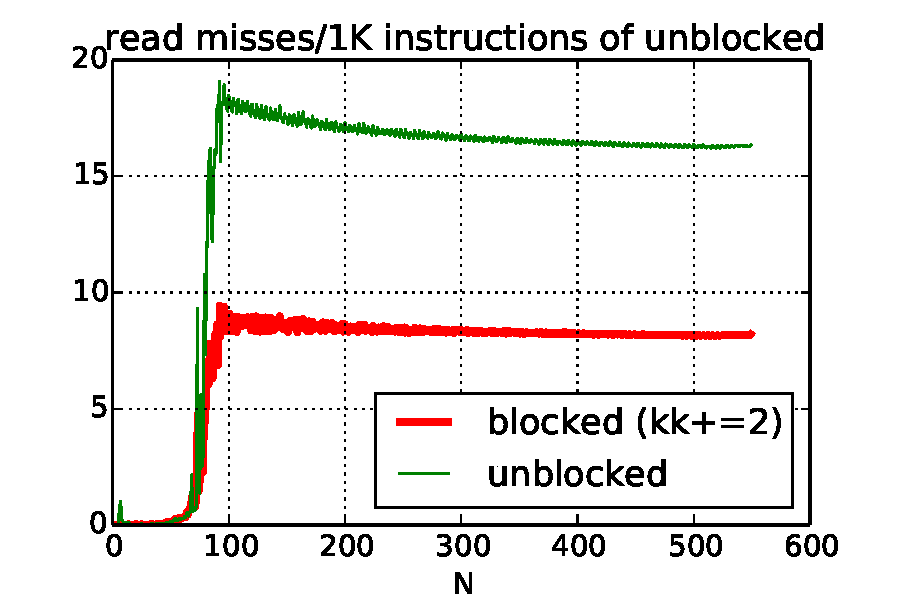
\includegraphics[width=0.8\textwidth]{../caching/k-kk-novec-block-read_miss_rate}
\end{frame}


\begin{frame}[fragile,label=cacheBlockBetter]{array usage (2 $k$ at a time)}
\begin{tikzpicture}
\draw[fill=yellow!10] (0, 0) rectangle (4, 4);
\draw[fill=yellow!10] (5, 0) rectangle (9, 4);
\draw[fill=yellow!10] (10, 0) rectangle ++(4, 4);
%\fill[green] (0.51, 3.49) rectangle (0.19, 3.81);
\begin{visibleenv}<3->
\fill[green] (2.99, 0.49) rectangle ++(0.31, 0.14);
\end{visibleenv}
%\fill[red] (0.5, 3.5) rectangle (0.2, 3.8) node[black,midway, above=5pt,fill=none,align=left] {$A_{ik}$ to $A_{i+1,k+1}$};
\fill[red] (3, 0.5) rectangle ++(0.3, 0.1)
    node[black,midway, above=5pt,fill=none,align=left] {$A_{ik}$ to $A_{i,k+1}$};
    \begin{visibleenv}<3,5>
        \draw[thick,blue] (2.7, 0.5) rectangle ++(0.7, 0.1);
    \end{visibleenv}
%\fill[green] (3.5, 0.0) rectangle (3.8, 4.0) node[black,midway,left,align=right,fill=none] {$A_{k0}$\\to\\$A_{k+1,N}$};
\begin{visibleenv}<3->
\fill[green] (5.0+0.0, 3.0) rectangle ++(4.0, 0.3) node[black,midway,below,align=right,fill=none] {$B_{k0}$ to $B_{k+1,N}$};
\end{visibleenv}
%\fill[red] (3.5, 0.8) rectangle (3.8, 0.9);
\fill[red] (5.0+0.5, 3.0) rectangle ++(0.1, 0.3)
    node[black,midway,right=5pt,fill=none,align=left,visible on=<1>]{$B_{ki}$ to $B_{k+1,i}$}
;
    \begin{visibleenv}<4,5>
        \draw[thick,blue] (5.0+0.3, 3.0) rectangle ++(0.7,0.15);
        \draw[thick,blue] (5.0+0.4, 3.15) rectangle ++(0.7,0.15);
    \end{visibleenv}
%\fill[green] (5.5, 0.0) rectangle (5.2, 4.0) node[black,midway,right,align=left,fill=none] {$B_{i0}$\\to\\$B_{i+1,N}$};
\begin{visibleenv}<3->
\fill[green] (10.0, 0.5) rectangle ++(4.0, 0.1) node[black,midway,right,align=left,fill=none] {$C_{i0}$ to $C_{iN}$};
\end{visibleenv}
    \begin{visibleenv}<5>
        \draw[thick,blue] (10.0+0.3, 0.5) rectangle ++(0.7,0.1);
    \end{visibleenv}
%\fill[red] (5.5, 0.8) rectangle (5.2, 0.9);
\fill[red] (10.0+0.5, 0.5) rectangle ++(0.1, 0.1)
    node[black,midway,right=5pt,fill=none,align=left,visible on=<1>]{$C_{ij}$};
    \begin{visibleenv}<1->
\node[anchor=north west,align=left] at (0.0,-0.5) {
for each kk: \\
\hspace{.5cm} for each i: \\
\hspace{1cm} \myemph<3->{for each j}: \\
\hspace{1.5cm} \myemph<1->{for k=kk,kk+1:} \\
\hspace{2cm} \myemph<1->{$C_{ij} += A_{ik}\cdot B_{kj}$} \\
};
\end{visibleenv}
\begin{visibleenv}<2>
\node[anchor=east,draw=red,ultra thick,align=left] at (15, -2) {
    within innermost loop \\
    good spatial locality in $A$ \\
    bad locality in $B$ \\
    good temporal locality in $C$
};
\end{visibleenv}
\begin{visibleenv}<3>
\node[anchor=east,draw=red,ultra thick,align=left] at (15, -2) {
    loop over $j$:
    \myemph<3>{better spatial locality} \\
    over $A$ than before; \\
    still good temporal locality for $A$ 
};
\end{visibleenv}
\begin{visibleenv}<4>
\node[anchor=east,draw=red,ultra thick,align=left] at (15.5, -2) {
    loop over $j$:
    spatial locality over $B$ is worse \\
    but probably not more misses \\
    cache needs to keep two cache blocks \\
    for next iter instead of one \\
    (probably has the space left over!)
};
\end{visibleenv}
\begin{visibleenv}<5>
\node[fill=white,anchor=east,draw=red,ultra thick,align=left] at (15.5, -2) {
    right now: only really care about \\
    keeping 4 cache blocks in $j$ loop \\
    ~ \\
    have more than 4 cache blocks? \\
    increasing $kk$ increment would use more of them
};
\end{visibleenv}
\end{tikzpicture}
\end{frame}



\subsection{explicit counting}
\begin{frame}{keeping values in cache}
    \begin{itemize}
        \item can't \textit{explicitly} ensure values are kept in cache
        \item \ldots but reusing values \textit{effectively} does this
            \begin{itemize}
                \item cache will try to keep recently used values
            \end{itemize}
            \vspace{.5cm}
        \item cache optimization ideas: choose what's in the cache
            \begin{itemize}
            \item for thinking about it: load values explicitly
            \item for implementing it: access only values we want loaded
            \end{itemize}
    \end{itemize}
\end{frame}


\subsection{how TLBs fit in the pipeline}
\usetikzlibrary{fit,positioning,shapes.callouts}

\begin{frame}{TLB and the MMU (1)}
\begin{tikzpicture}
\tikzset{>=Latex}
\node[minimum width=5cm,minimum height=2cm,draw,thick,align=center] (mmu) {MMU \\ \small (`page table walk' logic)};
\node[right=1.5cm of mmu,minimum width=5cm,minimum height=2cm,draw,thick] (cache) {L1 Cache/Memory};
\node[above=1.5cm of mmu,minimum width=5cm,minimum height=1cm,draw,thick] (tlb) {TLB};
    \node[left=1.5cm of mmu,align=right] (fromProgram) {address\\ from\\ program};
\draw[thick,<->] (mmu) -- (cache);
\draw[thick,<->] (mmu) -- (tlb);
    \draw[thick,->] (fromProgram) -- (mmu);
\end{tikzpicture}
\end{frame}

\begin{frame}{TLB and the MMU (2)}
\begin{tikzpicture}
\tikzset{
    >=Latex,
    pageNumber/.style={fill=blue!10,font=\fontsize{11}{12}\selectfont,inner sep=.5mm},
    pageOffset/.style={fill=green!10,font=\fontsize{11}{12}\selectfont,inner sep=.5mm},
    comp/.style={fill=yellow!10,font=\fontsize{12}{13}\selectfont},
    memAccess/.style={},
    ptMemAccess/.style={alt=<4>{red,very thick}},
    ifMiss/.style={draw=blue!50!black,alt={<1-2,6>{dashed,opacity=0.5}}},
    ifHit/.style={draw=violet!50!black,alt=<3-5>{dashed,opacity=0.5}},
    ifHitNoSkip/.style={draw=violet!50!black},
    checkValid/.style={alt=<6>{draw=red,very thick}},
}
\node[pageNumber] (addrLeft) {11 0101 01};
\node[anchor=west,pageOffset] (addrRight) at (addrLeft.east) {00 1101 1111};
\node[draw,comp,below=2cm of addrLeft,xshift=-.25cm,ifMiss] (timesPte) {$\times$ PTE size};
\draw[->,thick,ifMiss] (addrLeft.south -| timesPte.north) -- (timesPte);
\node[ifMiss,draw,very thick,below left=3cm and 1cm of addrLeft,label={[align=center,ifMiss,draw=none]north:page table\\base register}] (ptbr) {\tt 0x10000};
\node[draw,thick,above right=.6cm and .25cm of timesPte,fill=violet!10] (tlb) {TLB};
\draw[ifHitNoSkip,draw,very thick,->] (addrLeft) |- ([yshift=.4cm]tlb.north) -- (tlb.north);
\node[ifMiss,draw,comp] (plus) at (timesPte.south |- ptbr.west) {+};
\draw[->,thick,ifMiss] (timesPte) -- (plus);
\draw[->,thick,ifMiss] (ptbr) -- (plus);

\node[below=2cm of plus,fill=violet!10,draw,very thick,minimum height=1cm,minimum width=12cm,xshift=3cm] (cache) {data or instruction cache};
\node[pageNumber] (addrLeftFinal) at ([yshift=-1cm,xshift=7cm]plus) {1101 0011 11};
\draw[->,thick,memAccess,ifMiss,ptMemAccess] (plus) -- (cache.north -| plus.south);
\node[above right=1cm and 4cm of plus,align=center,draw,comp,checkValid] (check) {check valid \\ and permission bit};
\node[below=1cm of check,draw,comp] (split) {split PTE parts};
\draw[->,thick] (split) -- (check);
\draw[->,thick] ([xshift=1cm]check.north) -- ++(1cm, 1cm) node[above] {cause fault?};

\draw[ifHit,draw,very thick,->] (tlb.south) |- (split);
\draw[blue!50!black,->,thick] (split) -- (addrLeftFinal);

\node[anchor=west,pageOffset] (addrRightFinal) at (addrLeftFinal.east) {00 1101 1111};
\draw[very thick,green!50!black,densely dotted] ([xshift=1cm]addrRight.south) |- ([xshift=-.5mm,yshift=.5cm]split.north);
\draw[very thick,green!50!black,densely dotted,->] ([xshift=.5mm,yshift=.5cm]split.north) -| (addrRightFinal.north);

\node[inner sep=0mm,draw,label={[font=\fontsize{12}{13}\selectfont]south:physical address},fit=(addrLeftFinal) (addrRightFinal)] (addrFinal) {};

\node[inner sep=0mm,draw,label={[font=\fontsize{12}{13}\selectfont]north:virtual address},fit=(addrLeft) (addrRight)] (addr) {};

\draw[->,thick,memAccess] (addrFinal) -- (cache.north -| addrFinal.south);

\draw[ifMiss,->,very thick] (cache.north -| split.south) -- ++(0cm, 1cm) -| ([yshift=-.5cm,xshift=-.1cm]tlb.west) 
    -| ([xshift=-.4cm]tlb.west) -- (tlb.west);
\draw[->,thick,ifMiss,ptMemAccess] (cache.north -| split.south) -- (split.south);

%\begin{pgfonlayer}{bg}
%\node [fill=black!5,fit=(timesPte) (split),draw,line width=0.5mm,dashed,label={south:memory management unit (MMU)}] (mmu) {};
%\end{pgfonlayer}

\begin{visibleenv}<2>
\node[xshift=-4cm,above=0.5cm of cache,draw=red,ultra thick,fill=white,align=left] {TLB hit: TLB accesses replaces \\ page table access};
\end{visibleenv}


\begin{visibleenv}<4>
\node[xshift=-3cm,above=6cm of cache,draw=red,ultra thick,fill=white] {TLB miss: page table access happens};
\end{visibleenv}
\begin{visibleenv}<5>
\node[xshift=-1cm,above=6cm of cache,draw=red,ultra thick,fill=white] {TLB miss: TLB gets a copy of the page table entry};
\draw[red,->,very thick] (cache.north -| split.south) -- ++(0cm, 1cm) -| ([yshift=-.5cm,xshift=-.1cm]tlb.west) 
    -| ([xshift=-.4cm]tlb.west) -- (tlb.west);
\end{visibleenv}
\begin{visibleenv}<6>
\node[xshift=-3cm,above=2cm of cache,draw=red,ultra thick,fill=white,align=left] {on \textit{hit or miss} \\need to check permissions \\
    (read/kernel/etc.) \\
    but TLB only stores valid PTEs
};
\end{visibleenv}
\end{tikzpicture}
\end{frame}


\subsection{aside: TLB invalidation}
\begin{frame}{changing page tables}
\begin{itemize}
\item what happens to TLB when page table base pointer is changed?
    \begin{itemize}
    \item e.g. context switch
    \end{itemize}
\item most entries in TLB refer to things from \myemph{wrong process}
    \begin{itemize}
    \item oops --- read from the wrong process's stack?
    \end{itemize}
\vspace{.5cm}
\item<2-> option 1: \myemph{invalidate} all TLB entries
    \begin{itemize}
    \item side effect on ``change page table base register'' instruction
    \end{itemize}
\item<3-> option 2: TLB entries contain process ID
    \begin{itemize}
    \item set by OS (special register)
    \item checked by TLB in addition to TLB tag, valid bit
    \end{itemize}
\end{itemize}
\end{frame}

\begin{frame}{editing page tables}
\begin{itemize}
\item what happens to TLB when OS changes a page table entry?
\item most common choice: has to be handled \myemph{in software}
\vspace{.5cm}
\item<2-> invalid to valid --- nothing needed
    \begin{itemize}
    \item TLB doesn't contain invalid entries
    \item MMU will check memory again
    \end{itemize}
\item<2-> valid to invalid --- \myemph{OS needs to tell processor} to invalidate it
    \begin{itemize}
    \item special instruction (x86: {\tt invlpg})
    \end{itemize}
\item<2-> valid to other valid --- \myemph{OS needs to tell processor} to invalidate it
\end{itemize}
\end{frame}


\subsection{exercise: splitting for TLBs}
\subsubsection{1}
\begin{frame}{address splitting for TLBs (1)}
\begin{itemize}
\item my desktop:
\item 4KB ($2^{12}$ byte) pages; 48-bit virtual address
\item 64-entry, 4-way L1 data TLB
\vspace{.5cm}
\item TLB index bits?
\iftoggle{heldback}{}{
    \begin{itemize}\item<2->$64/4 = 16$ sets --- 4 bits\end{itemize}
}
\item TLB tag bits?
\iftoggle{heldback}{}{
    \begin{itemize}\item<2->$48-12=36$ bit virtual page number ---  $36-4=32$ bit TLB tag\end{itemize}
}
\end{itemize}
\end{frame}


\subsubsection{2}

\begin{frame}{address splitting for TLBs (2)}
\begin{itemize}
\item my desktop:
\item 4KB ($2^{12}$ byte) pages; 48-bit virtual address
\item 1536-entry ($3\cdot 2^9$), 12-way L2 TLB
\vspace{.5cm}
\item TLB index bits?
\iftoggle{heldback}{}{
    \begin{itemize}\item<2->$1536/12 = 128$ sets --- 7 bits\end{itemize}
}
\item TLB tag bits?
\iftoggle{heldback}{}{
    \begin{itemize}\item<2->$48-12=36$ bit virtual page number ---  $36-7=29$ bit TLB tag\end{itemize}
}
\end{itemize}
\end{frame}





\subsection{TLBs and context switches}
\begin{frame}{changing page tables}
\begin{itemize}
\item what happens to TLB when page table base pointer is changed?
    \begin{itemize}
    \item e.g. context switch
    \end{itemize}
\item most entries in TLB refer to things from \myemph{wrong process}
    \begin{itemize}
    \item oops --- read from the wrong process's stack?
    \end{itemize}
\vspace{.5cm}
\item<2-> option 1: \myemph{invalidate} all TLB entries
    \begin{itemize}
    \item side effect on ``change page table base register'' instruction
    \end{itemize}
\item<3-> option 2: TLB entries contain process ID
    \begin{itemize}
    \item set by OS (special register)
    \item checked by TLB in addition to TLB tag, valid bit
    \end{itemize}
\end{itemize}
\end{frame}

\begin{frame}{editing page tables}
\begin{itemize}
\item what happens to TLB when OS changes a page table entry?
\item most common choice: has to be handled \myemph{in software}
\vspace{.5cm}
\item<2-> invalid to valid --- nothing needed
    \begin{itemize}
    \item TLB doesn't contain invalid entries
    \item MMU will check memory again
    \end{itemize}
\item<2-> valid to invalid --- \myemph{OS needs to tell processor} to invalidate it
    \begin{itemize}
    \item special instruction (x86: {\tt invlpg})
    \end{itemize}
\item<2-> valid to other valid --- \myemph{OS needs to tell processor} to invalidate it
\end{itemize}
\end{frame}


